\documentclass{jknotes}
\usepackage{../joshkirklin}

\tikzset{
    partial ellipse/.style args={#1:#2:#3}{
        insert path={+ (#1:#3) arc (#1:#2:#3)}
    }
}

\setmathfont{Latin Modern Math}
\setmathfont{GFS NeoHellenic Math}[range=bfsfup/{greek,Greek}->it]
\setmathfont{GFS NeoHellenic Math}[range=sfup/{latin,Latin}->it]

\usetikzlibrary{intersections, pgfplots.fillbetween}

\begin{document}

\institution{Cambridge Part III Maths}
\title{Non-Newtonian Fluid Mechanics}
\lecturer{Eric Lauga}
\notetaker{Charles Powell}
\date{Michaelmas 2020}

\maketitle
\suggestionsspiel
\tableofcontents

\section{Introduction to Non-Newtonian Fluids}
\lecture{08/10/20}
Newtonian fluids are typically characterised by 2 material properties:
viscosity and density. We may also refer to Newtonian fluids as `simple
fluids'.


Non-Newtonian fluids may have many other material properties, for example
intrinisic time, length and stress scales, and an intrinsic orientation. They
often exhibit a mix of fluid and solid behaviour. We may also refer to
non-Newtonian fluids as `complex fluids'.


There are many examples of complex fluids readily apparent in our everyday
lives, for example sand (wet or dry) and mud; lava and glass, both of which
experience phase changes; ketchup; foam; paint; emulsions such as milk; liquid
crystals used in screens; blood on very small scales.


The goal of this course is to cover three main areas.
\begin{itemize}
	\item Phenomenology of non-Newtonian fluids -- how do they behave?
	\item Mathematical modelling -- how do we quantify the behaviour?
	\item Predictions (and limits) of models
\end{itemize}

\section{Summary of Newtonian Fluid Mechanics}
\subsection{Continuum approximation}
We describe fluids in terms of two main fields: \emph{density} $\rho(\symbf{x},t)$  and
\emph{velocity} $\symbf{u}(\symbf{x},t)$. We use the continuum approximation whereby the
fluid is assumed to be a continuum rather than made up of discrete fluid
particles. Under this assumption, the macroscopic properties of density and
velocity are well-defined as `averages' of infinitesimal volume elements. 

The velocity field is \emph{Eulerian}, meaning it is measured at a specific
point in space and time, as opposed to following a material element
(Lagrangian).

\subsection{Conservation of mass}

Conservation of mass can be expressed in the classical form of a conservation
equation as:
\begin{equation}
	\frac{\partial \rho}{\partial t} + \nabla \cdot \left[ \rho \symbf{u} \right]
	= 0
\end{equation}

Expanding the flux term, this may be expressed in a form which relates the
rate of change of density of a fluid element with the divergence of the
flow:
\begin{equation}
	\frac{\diffD{\rho}}{\diffD{t}} = -\rho \nabla \cdot \symbf{u}
\end{equation}

In this course we will assume that all fluids are incompressible, which is
expressed mathematically as:
\begin{equation}
	\frac{\diffD{\rho}}{\diffD{t}} = 0 \iff \nabla \cdot \symbf{u} = 0
\end{equation}

\subsection{Mechanical equilibrium}
Newton's second law, i.e. conservation of momentum is expressed for a fluid
using the \emph{Cauchy momentum equation}:
\begin{equation}
	\rho \frac{\diffD{\symbf{u}}}{\diffD{t}} = \rho \left[ \frac{\partial
	\symbf{u}}{\partial t} + \symbf{u} \cdot \nabla \symbf{u}\right] = \nabla \cdot
	\sigma + \symbf{F}
\end{equation}

where $\nabla \cdot \sigma$ are the surface forces acting on the fluid and
$\symbf{F}$ are body forces which we will assume to be negligible unless
otherwise stated.
 
The Cauchy momentum equation is valid for all continuum fluids. To close the
equation, we require an expression for $\sigma$.

\begin{defn}
The \emph{stress tensor} $\sigma$ is a symmetric second-rank tensor.
\begin{center}
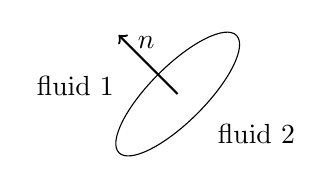
\begin{tikzpicture}
	\draw[rotate=45] (0,0) ellipse (30pt and 10pt);
	\draw[->, thick] (0,0) -- (-.75,.75);
	\node at (-0.4,0.65) {$\symbf{n}$};
	\node at (-1.3,0.1) {fluid 1};
	\node at (1,-0.5) {fluid 2};
\end{tikzpicture}
\end{center}
Physically, $\sigma_{ij}n_j$ is the $i\textsuperscript{th}$ component of the force per
unit area from the motion of fluid 1 on fluid 2, where $\symbf{n}$ is the
surface normal pointing into fluid 1.
\end{defn}

\subsection{Constitutive modelling}
The stress tensor is specified in terms of the deformation via \emph{constitutive
modelling}.

\begin{eg}{Newton's experiment\\}
Consider two parallel plates of area $A$ separated a distance $h$ by a fluid.
We consider the force $F$ required on the top plate to induce motion at speed
$U$. Note that there is no force perpendicular to the plates if the fluid is
Newtonian. This is not necessarily true for complex fluids.
\begin{center}
	\begin{tikzpicture}
		\begin{axis}[scatter/classes={a={mark=x,draw=black}},yticklabels={,,},xticklabels={,,},xlabel={$U/h$},ylabel={$F/A$},xmin=0,xmax=5,ymin=0,ymax=5]
		\addplot[scatter,only marks, scatter src = explicit symbolic]
		table[meta = label] {
			x y label 
			0.98 1 a
			1.5 1.48 a
			2 2.03 a
			2.43 2.39 a
			3.03 3.01 a
			3.45 3.55 a
			4.01 4 a
		};
		\addplot[no marks, black, dashed]{x};
	\end{axis}
	\end{tikzpicture}
\end{center}

From experiment, we find $\sigma = F/A \propto U/h$. Note that $U/h$ has
dimensions of time$^{-1}$. We define the \emph{shear rate} $\srate =
U/h$ and the \emph{viscosity} $\eta$ via $\sigma = \eta \srate$.
Viscosity is a constant material property, for example in water $\eta =
10^{-3}\, \text{Pa}\cdot\text{s}$.

\end{eg}

We can now generalise for all Newtonian flows. We start by separating out an
isotropic component of the shear tensor:
\begin{equation}
	\sigma_{ij} = -p \delta_{ij} + \tau_{ij}
\end{equation}
where $p$ is the \emph{dynamic pressure} and $\tau$ is the \emph{deviatoric
stress}. The deviatoric stress may be a function of $u_i, \frac{\partial u_i}{\partial
x_j}, \dots$; local or non-local in time or space; or a function of other
material properties and parameters. For Newtonian fluids, we make five
assumptions.

\begin{enumerate}
	\item Galilean invariance: the deviatoric stress cannot depend on $u_i$
	\item Instaneous response: there is no dependence on the history of
		deformation
	\item Locality: no dependence on second or higher spatial derivatives
	\item Linearity: $\tau_{ij}$ is linearly related to $\frac{\partial
		u_m}{\partial x_n}$
	\item Isotropy: the relationship is independent of reference frame, i.e.
		isotropic
\end{enumerate}

We can satisfy 1, 2, 3, and 4 by writing
\begin{equation}
	\tau_{ij} = A_{ijkl}\frac{\partial u_k}{\partial x_l}
\end{equation}
where $A_{ijkl}$ is a fourth rank tensor. Using the form of the most general
isotropic fourth rank tensor we may enforce isotropy.
\begin{equation}
	A_{ijkl} = A \delta_{ij} \delta_{kl} + B \delta_{ik}\delta_{jl} + C
	\delta_{il}\delta_{jk}
\end{equation}

Since $\sigma$ is symmetric, $\tau$ is symmetric, therefore $A_{ijkl} =
A_{jikl}$. This requires $B = C \equiv \eta$. Thus
\begin{equation}
	\begin{aligned}
		\tau_{ij} &= A\delta_{ij} \frac{\partial u_k}{\partial x_k} + \eta
		\left( \frac{\partial u_i}{\partial x_j} + \frac{\partial
		u_j}{\partial x_i} \right) \\
		&= \eta \left( \frac{\partial u_i}{\partial x_j} + \frac{\partial
		u_j}{\partial x_i} \right) \\
		&= 2 \eta e_{ij}
	\end{aligned}
\end{equation}

since $\frac{\partial u_k}{\partial x_k} = \nabla \cdot \symbf{u} = 0$. Note
$e = \frac{1}{2}\left(\nabla \symbf{u} + (\nabla \symbf{u})^T\right)$ is the
\emph{rate of strain} tensor. This is the \emph{Newtonian constitutive
	relationship}. 
	
\begin{defn}
	To exclude the factors of $2$ we define the \emph{shear rate}
	$\srate_{ij} = 2 e_{ij}$ so that $\tau_{ij} = \eta
	\srate_{ij}$.
\end{defn}

Combining the Cauchy momentum equation and Newtonian constitutive relationship
yields the \emph{Navier-Stokes equations}
\begin{equation}
	\rho \frac{\diffD{\symbf{u}}}{\diffD{t}} = - \nabla p + \eta \nabla^2 \symbf{u}
\end{equation}

Consider a general body with intrinsic length scale $L$, velocity length scale
$U$ and unsteady motion frequency scale $\omega$. Two dimensionless numbers
are used to quantify the importance of inertia:
\begin{equation}
	\text{Re} = \frac{\rho U L}{\eta}, \hspace{2em} \text{Re}_\omega =
	\frac{\rho \omega L^2}{\eta}
\end{equation}

We will assume throughout this course that $\text{Re} \ll 1$ and
$\text{Re}_\omega \ll 1$ unless otherwise stated. In this no-inertia limit,
the Navier-Stokes equations simplify to the \emph{Stokes equations}. For a
general fluid these are:
\begin{equation}
	\nabla \cdot \sigma = 0
\end{equation}

Using the Newtonian constitutive relationship, the Stokes equations are:
\begin{equation}
	\symbf{0} = -\nabla p + \eta \nabla^2 \symbf{u}
\end{equation}

\begin{eg}{Newton's experiment revisited\\}
	We will apply the above theory to Newton's experiment and show the same
	results are obtained.

	\begin{center}
		\begin{tikzpicture}
			\node at (0,2) {$y = h$};
			\draw (0.6, 2) -- (5, 2);
			\node at (0,0) {$y=0$};
			\draw (0.6, 0) -- (5,0);
			\node at (2.5, 2.5) {$U$};
			\draw[->, thick] (2.15, 2.25) -- (2.85, 2.25);
			\draw[->] (1,0.5) -- (1.6, 0.5) node[midway,below] {$\hat{\symbf{x}}$};
			\draw[->] (1,0.5) -- (1, 1.1) node[midway, left] {$\hat{\symbf{y}}$};
		\end{tikzpicture}
	\end{center}

	Assume the flow is unidirectional: $\symbf{u} = u(y) \hat{\symbf{x}}$. The
	Stokes equations become
	\begin{equation}
	\begin{cases}
		\frac{\partial p}{\partial x} = \eta \frac{\partial^2 u}{\partial y^2}
		& = \text{const.}
		\\
		\frac{\partial  p}{\partial y} = 0 & \implies p=p(x)
	\end{cases}
	\end{equation}

	Assuming there is no net pressure drop, $p = p(x) \equiv 0$. Applying the
	boundary conditions we find 
	\begin{equation}
		u(y) = Uy/h \implies \srate = U/h
	\end{equation}
	as before. This is a \emph{shear} or \emph{Couette} flow.
\end{eg}

\lecture{13/10/20}
\section{Phenomenology}

There are four distinguishing properties of non-Newtonian fluids which differ
to Newtonian fluids.

\subsection{Shear-dependent viscosity}
Newtonian fluids have a constant viscosity $\eta$ which is a constant of
proportionality between shear stress $\sigma$ and shear rate $\srate$.
For a complex fluid, $\eta$ is \emph{not} constant. We re-define viscosity as
an implicit function of shear rate.
\begin{defn}
	Viscosity is defined via $\eta \equiv \frac{\sigma}{\srate} =
	\eta(\srate)$.
\end{defn}

We can broadly categorise complex fluids into two types: \emph{shear thinning}
and \emph{shear thickening} fluids.

\begin{center}
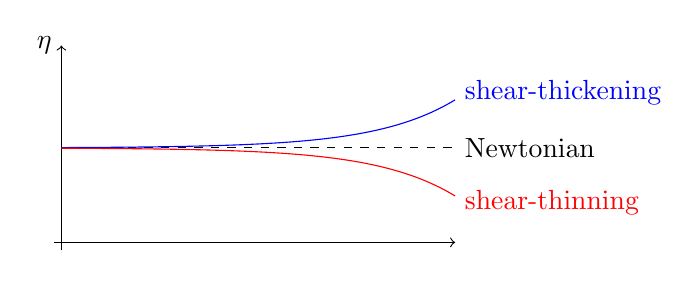
\begin{tikzpicture}
	\draw[->] (-0.1,0) -- (5,0) node[below] {$\srate$};
	\draw[->] (0,-0.1) -- (0,2.5) node[left] {$\eta$};
	\draw[dashed] (0,1.2) -- (5, 1.2) node[right] {Newtonian};
	\draw[smooth,samples=100,domain=0:5,blue] plot(\x, {1.2+0.5*exp(\x-4.8)});
	\draw[smooth,samples=100,domain=0:5,red] plot(\x, {1.2-0.5*exp(\x-4.8)});
	\draw (5, 1.9) node[right,blue] {shear-thickening};
	\draw (5, 0.5) node[right,red] {shear-thinning};
\end{tikzpicture}
\end{center}

Examples of shear-thinning fluids are polymer suspensions; paint; blood. These
complex fluids have $\frac{\partial \eta}{\partial \srate} < 0$.

Examples of shear-thickening fluids are: cornstarch in water; suspesions of
colloidal particles. These complex fluids have $\frac{\partial \eta}{\partial
\srate} > 0$.

\begin{defn}
	The zero-shear rate viscosity is $\eta_0 = \lim_{\srate \to 0}
	\eta$.
\end{defn}

Note that some complex fluids have approximately constant viscosity (Boger
fluids).

\subsection{Fluid memory}
Consider a step-shear flow, that is, Newton's experiment where the top place
impulsively starts motion at $t=0^+$. The response of a Newtonian fluid is on
an inertial timescale $\tau \sim h^2/\nu$ which is almost instantaneous,
whilst a non-Newtonian fluid takes time to respond to adjust to the change in
deformation: the jump occurs over some \emph{relaxation timescale} $\lambda$.

\begin{center}
	\begin{tikzpicture}
		\draw[->] (0,-0.1) -- (0,2.5) node[left] {$\srate$};
		\draw[->] (-0.1,0) -- (5,0) node[below] {$t$};
		\draw (1, -0.1) -- (1, 0.1) node[below] {$t=0$};
		\draw[blue,thick] (0,0) -- (1, 0);
		\draw[blue,thick] (1, 1.2) -- (5, 1.2);
		\draw[blue] (5, 1.4) node[right] {newtonian};
		\draw[red] (5, 1) node[right] {complex};
	\end{tikzpicture}
	\qquad
	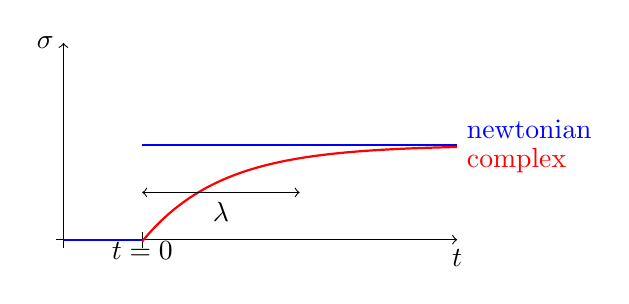
\begin{tikzpicture}
		\draw[->] (0,-0.1) -- (0,2.5) node[left] {$\sigma$};
		\draw[->] (-0.1,0) -- (5,0) node[below] {$t$};
		\draw (1, -0.1) -- (1, 0.1) node[below] {$t=0$};
		\draw[blue,thick] (0,0) -- (1, 0);
		\draw[blue,thick] (1, 1.2) -- (5, 1.2);
		\draw[red, thick, smooth, samples=100, domain=1:5] plot(\x, {1.2 -
		exp(-\x+1.2)});
		\draw[blue] (5, 1.4) node[right] {newtonian};
		\draw[red] (5, 1) node[right] {complex};
		\draw[<->] (1, 0.6) -- (3, 0.6) node[below, midway] {$\lambda$};
	\end{tikzpicture}
\end{center}

The relationship between stress and deformation is \emph{history dependent}.
Impulsively removing the applied shear (i.e. the plate impulsively comes to
rest) results in \emph{stress relaxation} with $\sigma \sim e^{-t/\lambda}$.

\begin{center}
	\begin{tikzpicture}
		\draw[->] (0,-0.1) -- (0,2.5) node[left] {$\srate$};
		\draw[->] (-0.1,0) -- (5,0) node[below] {$t$};
		\draw (2, -0.1) -- (2, 0.1);
		\draw[blue,thick] (0,1.2) -- (2, 1.2);
		\draw[blue,thick] (2, 0) -- (5, 0);
		\draw[blue] (5, 1.4) node[right] {Newtonian};
		\draw[red] (5, 1) node[right] {complex};
	\end{tikzpicture}
	\qquad
	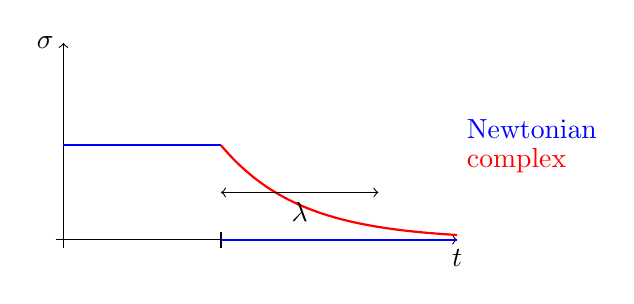
\begin{tikzpicture}
		\draw[->] (0,-0.1) -- (0,2.5) node[left] {$\sigma$};
		\draw[->] (-0.1,0) -- (5,0) node[below] {$t$};
		\draw (2, -0.1) -- (2, 0.1);
		\draw[blue,thick] (0,1.2) -- (2, 1.2);
		\draw[blue,thick] (2, 0) -- (5, 0);
		\draw[red, thick, smooth, samples=100, domain=2:5] plot({\x},
		{1.2*exp(-\x+2)});
		\draw[blue] (5, 1.4) node[right] {Newtonian};
		\draw[red] (5, 1) node[right] {complex};
		\draw[<->] (2, 0.6) -- (4, 0.6) node[below, midway] {$\lambda$};
	\end{tikzpicture}
\end{center}

The reverse is also true. Imposing a stress $\sigma$ and measuring the
deformation $\srate$, complex fluids in general wil have a
history-dependent response. This is called \emph{strain retardation} and
$\lambda'$ is the \emph{retardation timescale}.

\subsection{Normal stress differences}
In Newton's experiment, a Newtonian fluid exerts no normal force $F_N$ on the moving
plate, since linearity and reversibility ($U \to -U$) impies $F_N = -F_N
\equiv 0$. We previously calculated 
\begin{equation}
	\symbf{u} = \frac{Uy}{h}\hat{\symbf{x}}, \hspace{2em} \srate = \frac{U}{h}
\end{equation}
Thus in the Newtonian case the stress tensor has the form
\begin{equation}
	\sigma = \begin{pmatrix}
		-p_0 & \eta \srate & 0 \\
		\eta \srate & -p_0 & 0 \\
	0 & 0 & -p_0 \end{pmatrix}
\end{equation}
where $p_0$ is the external pressure. Note that the normal stresses are equal
and constant.

In the non-Newtonian case we have
\begin{equation}
	\sigma = \begin{pmatrix}
		\sigma_{xx} & \eta)(\srate) \srate & 0 \\
		\eta(\srate) \srate & \sigma_{yy} & 0 \\
	0 & 0 & \sigma_{zz} \end{pmatrix}
\end{equation}
where in general normal stresses are not equal and not constant. Normal
stresses include the external pressure, so the relevant quantity is the
difference between normal stresses.
\begin{defn}
	The first and second \emph{normal stress differences} are
	\begin{equation}
		N_1 = \sigma_{xx} - \sigma_{yy}, \hspace{2em} N_2 = \sigma_{yy} -
		\sigma_{zz}
	\end{equation}
\end{defn}

Note the following.
\begin{itemize}
	\item For a Newtonian fluid, $N_1 = N_2 = 0$
	\item Polymeric fluids (for example) have $N_1 > 0, N_2 < 0, \left|
		N_2/N_1 \right| \sim 0.1$
	\item $N_1$ and $N_2$ are defined only for steady shear flow
	\item $N_1$ and $N_2$ will, in general, depend on $\srate$
	\item Boger fluids have constant viscosity but they have non-zero $N_1$
		and $N_2$
\end{itemize}

Reversibility implies $N_1$ and $N_2$ have to be \emph{even} functions of
$\srate$. In the limit $\srate \to 0$, i.e. the Newtonian limit,
we should have $N_1 \to 0, N_2 \to 0$. Thus the Taylor expansion of $N_1, N_2$
near $\srate = 0$ is
\begin{equation}
	N_{1,2} = A_{1,2}\srate^2 + B_{1,2}\srate^4 + \dots
\end{equation}

\begin{defn}
	The \emph{normal stress coefficients} are
	\begin{equation}
		\Psi_1 = \frac{N_1}{\srate^2}, \hspace{2em} \Psi_2 =
		\frac{N_2}{\srate^2}
	\end{equation}
\end{defn}

The physical consequence of having normal stress differences is the
introduction of elastic tension along flow streamlines.

Suppose $\sigma_{xx} = -p$. Thus compression $p > 0 \implies \sigma_{xx} < 0$
and $N_1 > 0 \implies \sigma_{xx} > 0$ which can be thought of as `negative
pressure' which acts as tension. An intuitive example is stretching of polymer
molecules. This has many consequences on experiments and flow behaviour.

\begin{eg}
	Two examples of the consequences of normal stress differences are as
	follows.
	\begin{enumerate}
		\item Rod-climbing (\emph{Weissenberg effect}).
			\begin{center}
				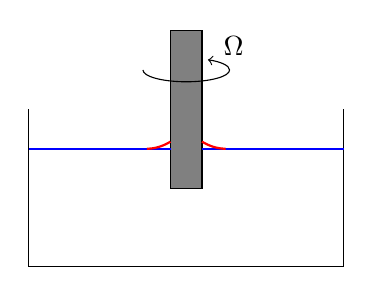
\begin{tikzpicture}
					\draw (-2, 0) -- (2, 0);
					\draw (-2,0) -- (-2, 2);
					\draw (2,0) -- (2, 2);
					\draw[fill=gray] (-0.2,1) rectangle ++ (0.4, 2);
					\draw[blue,thick] (-2, 1.5) -- (-0.2, 1.5);
					\draw[blue,thick] (2, 1.5) -- (0.2,1.5);
					\draw[->] (0, 2.5) [partial ellipse = -180:60:0.55 and
					0.15];
					\draw (0.35, 2.8) node[right] {$\Omega$};
					\draw[red, thick, smooth, samples=100, domain=-0.5:-0.2]
					plot(\x, {1.5+(\x+0.5)^2});
					\draw[red, thick, smooth, samples=100, domain=0.2:0.5]
					plot(\x, {1.5+(\x-0.5)^2});
				\end{tikzpicture}
			\end{center}
			Consider a vertical rod rotating at a constant rate $\Omega$
			placed into a fluid. In a Newtonian fluid, viscous enough for
			Stokes equations to apply, there is no change in the position of
			the interface (blue).

			In a non-Newtonian fluid, the interface climbs up the rod (red).
			This is due to elastic tension: rotation creates circular
			streamlines. Tension along circles creates \emph{hoop stress}
			which `squeezes' the fluid and thus climbs up the rod.

		\item  Particle migration in a pipe flow.
			\begin{center}
				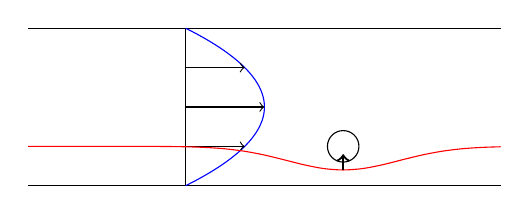
\begin{tikzpicture}
					\draw (-3, 1) -- (3, 1);
					\draw (-3, -1) -- (3, -1);
					\draw (-1, -1) -- (-1, 1);
					\draw[smooth, domain=-1:1, blue, variable=\y] plot ({-\y * \y}, {\y});
					\draw[->] (-1, 0) -- (0, 0);
					\draw[->] (-1, 0.5) -- (-0.25, 0.5);
					\draw[->] (-1, -0.5) -- (-0.25, -0.5);
					\draw (1, -0.5) circle (0.2);
					\draw[smooth,domain=-3:3,red] plot ({\x},
					{-0.5-0.3*exp(-(\x-1)^2)});
					\draw[thick,->] (1,-0.8) -- (1, -0.6);
				\end{tikzpicture}
			\end{center}
			In the case of Newtonian Stokes flow, the flow has no component
			perpendicular to the walls so a particle remains the same distance
			from the wall as it moves along the pipe. In the non-Newtonian
			case, hoop stress caused by curved streamlines lifts the particle
			away from the wall.
	\end{enumerate}
\end{eg}

\subsection{Extensional Viscosity}
A shear flow is a \emph{weak flow}: there is algebraic growth of distances
between particles. In a \emph{strong flow}, distances grow exponentially.

Consider a fluid with extension in the $x$ and $y$ directions and compression
in the $z$ direction: $\symbf{u} +
\dot{\varepsilon}\left(\frac{1}{2}x,\frac{1}{2}y, -z\right)$. We call
$\dot{\varepsilon}$ the \emph{extension rate}. Note that this flow is
incompressible. The shear rate tensor is
\begin{equation}
	\symbfsf{\srate} = \dot{\varepsilon}\begin{pmatrix} 1 & 0 & 0 \\ 0 &
	1 & 0 \\ 0 & 0 & -2 \end{pmatrix}
\end{equation}

In the Newtonian case, the shear rate tensor is
\begin{equation}
	\symbfsf{\sigma} = \begin{pmatrix}
		-p_0 + \eta \dot{\varepsilon} & 0  & 0 \\
		0 & -p_0 + \eta \dot{\varepsilon} & 0 \\
		0 & 0 & -p_0 -2 \eta \dot{\varepsilon} 
	\end{pmatrix}
\end{equation}

\begin{defn}
	The \emph{extensional viscosity} is
	\begin{equation}
		\eta_{\text{ext}} = \frac{\sigma_{xx}-\sigma_{zz}}{\dot{\varepsilon}}
	\end{equation}
	which has units of viscosity.
\end{defn}

Thus for the Newtonian fluid, $\eta_{\text{ext}} = 3\eta$ which is constant. 
\begin{defn}
	The \emph{Troutou ratio} is 
	\begin{equation}
		\text{Tr} = \frac{\eta_{\text{ext}}}{\eta}
	\end{equation}
\end{defn}

By the above calculations, Newtonian fluids have $\text{Tr} = 3$.
Non-Newtonian fluids tend to have $\text{Tr} \gg 1$ in some range of shear
rates. Thus complex fluids have a very different response to strong flows
compared with weak flows.

\begin{center}
	\begin{tikzpicture}
		\draw[thick,->] (-0.1, 0) -- (5, 0) node[below] {$\dot{\varepsilon}$};
		\draw[thick,->] (0, -0.1) -- (0, 3) node[left] {Tr};
		\draw[dashed] (-0.1, 1) -- (5, 1);
		\draw (-0.1, 1) node[left] {$3$};
		\draw[smooth,blue,domain=0:5] plot({\x},{1+1/(0.5+exp(-2*(\x-3)))});
		\draw (5, 3) node[above] {$\text{Tr} \gg 1$};
	\end{tikzpicture}
\end{center}

\lecture{15/10/20}
\section{Generalised Newtonian Fluids}

We will focus on steady flows and fluids which are \emph{inelastic}. We will
find how to incorporate shear-dependent viscosity into the constitutive
relationship. One way is to generalise the Newtonian constitutive
relationship to
\begin{equation}
	\symbfsf{\sigma} = -p \symsf{1} +
	\eta(\symbfsf{\srate})\symbfsf{\srate}
\end{equation}
where $\eta(\symbfsf{\srate})$ is found empirically. These are called
\emph{generalised Newtonian fluids} (GNF).

We have a scalar function $\eta$ of a tensor $\symbfsf{\srate}$, which is
not in general coordinate invariant. Thus $\eta$ must be a function of the
\emph{invariants} of $\symbfsf{\srate}$. A rank $2$ tensor in $3$
dimensions has $3$ invariants. These are combinations of trace, determinants,
and eigenvalues. We choose as the three invariants:
\begin{equation}
	\trace{\symbfsf{\srate}}, \hspace{2em} \trace{\symbfsf{\srate} \cdot
	\symbfsf{\srate}}, \hspace{2em} \trace{\symbfsf{\srate} \cdot
\symbfsf{\srate} \cdot \symbfsf{\srate}}
\end{equation}

We always have $\trace{\symbfsf{\srate}} = 0$ because the flow is incompressible:
\begin{equation}
	\trace{\symbfsf{\srate}} = \srate_{ii} = \frac{\partial u_i}{\partial x_i} +
	\frac{\partial u_i}{\partial x_i} = 2\nabla \cdot \symbf{u} = 0
\end{equation}

Consider a simple shear flow $\symbf{u} = \srate y \hat{\symbf{x}}$. Then
\begin{equation}
	\begin{aligned}
		\symbfsf{\srate} &= \begin{pmatrix} 0 & \srate & 0 \\ \srate & 0 & 0 \\
		0 & 0 & 0 \end{pmatrix} \\
			\symbfsf{\srate}\cdot\symbfsf{\srate} &= \begin{pmatrix} \srate^2 &
			0 & 0 \\ 0 & \srate^2 & 0 \\ 0 & 0 & 0 \end{pmatrix} \\
			\symbfsf{\srate}\cdot\symbfsf{\srate}\cdot\symbfsf{\srate} &=
			\begin{pmatrix} 0 & \srate^3 & 0 \\ \srate^3 & 0 & 0 \\
			0 & 0 & 0 \end{pmatrix}
		\end{aligned}
\end{equation}

Thus $\trace{\symbfsf{\srate}\cdot\symbfsf{\srate}\cdot\symbfsf{\srate}} = 0$ and
$\trace{\symbfsf{\srate}\cdot\symbfsf{\srate}} = 2\srate^2$. We assume all flows
are approximately steady shear flow. Then
$\trace{\symbfsf{\srate}\cdot\symbfsf{\srate}}$ is the only non-zero invariant
and $\eta(\symbfsf{\srate}) =
\eta(\trace{\symbfsf{\srate}\cdot\symbfsf{\srate}})$.

\begin{defn}
	The \emph{magnitude of shear rate} is
	\begin{equation}
		\srate \equiv
		\left(\frac{\trace{\symbfsf{\srate}\cdot\symbfsf{\srate}}}{2}\right)^{1/2}
		= \left(\frac{\symbfsf{\srate} : \symbfsf{\srate}}{2}\right)^{1/2}
	\end{equation}
	Note that $\srate \ge 0$ and for a simple shear flow the magnitude of
	shear rate $\srate = \abs{\srate}$ which is the shear rate from steady
	shear flow. Thus the definitions coincide.
\end{defn}

Note the second invariant $\trace{\symbfsf{\srate}\cdot\symbfsf{\srate}} =
\symbfsf{\srate}:\symbfsf{\srate} \ge 0$ and is zero only when there is no
deformation (since $\symbfsf{\srate}:\symbfsf{\srate}$ is proportional to
viscous dissipation), i.e. rigid body motion.

Recall for a simple shear flow, the shear stress is $\sigma =
\eta(\srate)\srate$, thus the above definitions agree with measurements of
shear-dependent viscosity.

\subsection{Power-law fluids}
There are many choices for the function $\eta(\srate)$ for a generalised
Newtonian fluid. Here, we choose a \emph{power-law}
\begin{equation}
	\eta(\srate) \equiv \kappa \srate^{n-1}
\end{equation}
where $\kappa > 0$ and $n \in \ZZ$ is the \emph{power-index} of the fluid.
Note $n=1$ for a Newtonian fluid. For dimensional consistency, we require
$\left[\kappa\right] = \text{Pa}\cdot\text{s}^n$.

\begin{center}
	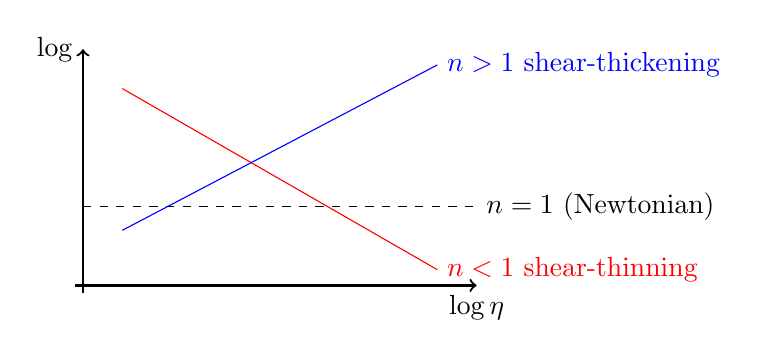
\begin{tikzpicture}
		\draw[thick,->] (-0.1, 0) -- (5, 0) node[below] {$\log \eta$};
		\draw[thick,->] (0, -0.1) -- (0, 3) node[left] {$\log \srate$};
		\draw[dashed] (0,1) -- (5, 1) node[right] {$n=1$ (Newtonian)};
		\draw[red] (0.5, 2.5) -- (4.5, 0.2) node[right] {$n < 1$
		shear-thinning};
		\draw[blue] (0.5, 0.7) -- (4.5, 2.8) node[right] {$n >1$
		shear-thickening};
	\end{tikzpicture}
\end{center}

Note that in the limit $\srate \to 0$, we cannot define a zero-shear rate
viscosity $\eta_0$ unless $n=1$. Thus the model is problematic at small shear
rates. The model is appropriate only for a finite range of shear rates.

\begin{eg}
	Newton's experiment with a power-law fluid. We assume there are no
	external pressures, and the flow is unidirectional: $\symbf{u} =
	u(y)\hat{\symbf{x}}$. We have
	\begin{equation}
		\symbfsf{\srate} = \begin{pmatrix} 0 & \frac{\partial u}{\partial y} &
			0 \\ \frac{\partial  u}{\partial y} & 0 & 0 \\ 0 & 0 & 0
		\end{pmatrix}
	\end{equation}

	Then the magnitude of shear rate $\srate = \abs{\frac{\partial u}{\partial
	y}}$. To find the flow, we use the Cauchy equation in 2D:
	\begin{equation}
		\begin{aligned}
			\frac{\partial p}{\partial y} &= 0 \\
			\frac{\partial p}{\partial x} &= \frac{\partial \sigma_{xy}}{\partial y} 
		\end{aligned}
	\end{equation}
	since $\sigma_{xy}$ is the only non-zero component of the shear stress.
	The first equation implies $p = p(x)$ only, which combined with the second
	implies $\sigma_{xy} = \text{const.}$. Note we have not used the
	constitutive relationship yet: this is true for all GNFs. We have
	\begin{equation}
		\sigma_{xy} = \kappa \srate^{n-1} \srate = \kappa \srate^n = \kappa
		\abs{\frac{\partial u}{\partial y}}^n = \text{const.}
	\end{equation}

	Thus $u_y$ is constant, i.e. $u$ is linear in $y$, as with a Newtonian
	fluid. 
\end{eg}

If $\eta(\srate)\srate = \sigma$ is a one-to-one function of $\srate$ then the
result is the same: $u$ varies linearly. A Couette flow $\symbf{u} = Uy/h
\hat{\symbf{x}}$ is a \emph{viscometric flow}: this flow is realised for all
constitutive relationships provided $\sigma$ is indeed a one-to-one function
of $\srate$.

How do experimentally measure $\eta(\srate)$? One method is a \emph{shear flow
rheometer}:
\begin{enumerate}
	\item Impose $\srate$, measure $\sigma$ (or vice versa)
	\item Measure $\eta = \sigma/\srate$
	\item Repeat varying $\srate$ or $\sigma$
\end{enumerate}

\subsubsection{Pipe flow of a power-law fluid}
\label{sec:pipe}
Consider axisymmetric pressure-driven flow in a pipe of a power-law GNF. If
the fluid was Newtonian, we would get Poiseuille flow with a parabolic flow
profile.

\begin{center}
\begin{tikzpicture}
	\draw (0,0) ellipse (0.6 and 1);
	\draw (0,-1) -- (8,-1);
	\draw (0, 1) -- (8,1);
	\draw (8,0) [partial ellipse = -90:90:0.6 and
	1];
	\draw[dashed] (8,0) [partial ellipse = 90:270:0.6 and
	1];
	\draw[thick,blue,->] (4,0) -- (6, 0) node[right] {flow};
	\draw (-2, 0) node {$p_0 + \Delta p$};
	\draw (10, 0) node {$p_0$};
	\draw[->] (0,0) -- (0,1) node[midway,right] {$R$};
	\draw[<->] (0,-1.5) -- (8,-1.5) node[midway, below] {$L$};
\end{tikzpicture}
\end{center}

We will use cylindrical coordinates $(r,\theta,z)$ and assume the flow is
unidirectional: $\symbf{u} = u(r)\hat{\symbf{z}}$. Then
\begin{equation}
	\symbfsf{\srate} = \begin{pmatrix} 0 & 0 & \frac{\partial u}{\partial r} \\
	0 & 0 & 0 \\ \frac{\partial u}{\partial r} & 0 & 0 \end{pmatrix}
\end{equation}

The magnitude of shear rate $\srate = \abs{\frac{\partial u}{\partial r}}$.
The Cauchy equations in cylindrical coordinates are
\begin{equation}
	\begin{aligned}
		\frac{\partial p}{\partial r} &= 0 \\
		\frac{\partial p}{\partial \theta} &= 0 \\
		\frac{\partial p}{\partial z} &= \frac{1}{r} \frac{\partial}{\partial
		r} \left( r \sigma_{rz}\right)
	\end{aligned}
\end{equation}

since $\sigma_{rz}$ is the only non-zero component of shear stress. The first
two equations imply $p = p(z)$. Then $\frac{\partial p}{\partial z}$ is a
function of $z$ only, but the RHS is a function of $r$ only. Thus each
must be constant. Then
\begin{equation}
	\frac{\partial p}{\partial z} = -\frac{\Delta p}{L} \implies \sigma_{rz} =
	-\frac{\Delta p}{2L} r + \frac{A}{r}
\end{equation}

The $A/r$ term is singular at $r=0$ thus $A \equiv 0$. Note these results are
true for all guids - we have not yet used the fact this is a power-law fluid.

Denote the \emph{magnitude of wall shear stress} as $\sigma_w$. In this case,
$\sigma_w = \frac{\Delta p}{2L}R$.  To find the flow field, we need the
constitutive relationship. For a GNF we have
\begin{equation}
	\sigma_{rz} = \eta\left(\abs{\frac{\partial u}{\partial r}}\right)
	\frac{\partial u}{\partial r} = -\frac{\Delta p}{2L} r
\end{equation}

We expect $u$ to be at maximum when $r=0$, so expect $\frac{\partial
u}{\partial r} < 0$. Thus $\abs{u_r} = -u_r$. For a power-law fluid, $\sigma =
\kappa \srate^n$, thus
\begin{equation}
	\begin{aligned}
		\kappa \abs{\frac{\partial u}{\partial r}}^n &= \frac{\Delta p}{2L} r
		\\
		\implies \abs{\frac{\partial u}{\partial r}} &= \left(\frac{\Delta p}{2
		L \kappa}\right)^{1/n} r^{1/n} = -\frac{\partial u}{\partial r} \\
		\implies u(r) &= C - \left(\frac{\Delta p}{2 L \kappa}\right)^{1/n}
		\frac{n}{n+1} r^{\frac{n+1}{n}}
	\end{aligned}
\end{equation}

Enforcing no-slip boundary conditions on the pipe wall $u(R) = 0$ and
re-writing in terms of the wall shear stress we have
\begin{equation}
	u(r) = \left(\frac{\sigma_w}{\kappa R}\right)^{1/n} \frac{n}{n+1}\left(
	R^{\frac{n+1}{n}} - r^{\frac{n+1}{n}}\right)
\end{equation}

We can calculate the mean flow speed $\bar{U}$:
\begin{equation}
	\bar{U} \equiv \frac{1}{\pi R^2} \iint u \, \diffd S = \frac{2}{R^2}
	\int_0^R ru(r) \, \diffd r = \left(\frac{\sigma_w}{\kappa}\right)^{1/n}
	\frac{nR}{3n+1}
\end{equation}

Finally, we can rewrite the solution as flow relative to the mean flow speed:
\begin{equation}
	\frac{u(r)}{\bar{U}} = \frac{3n+1}{n+1} \left[ 1-
	\left(\frac{r}{R}\right)^{\frac{n+1}{n}}\right]
\end{equation}

\begin{center}
	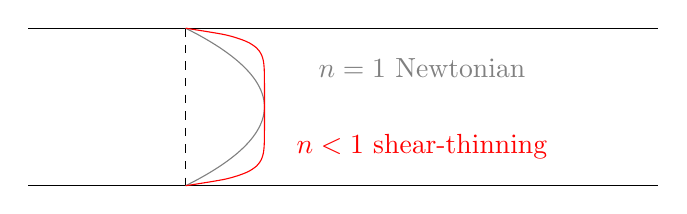
\begin{tikzpicture}
		\draw (0, 1) -- (8, 1);
		\draw (0, -1) -- (8, -1);
		\draw[dashed] (2,1) -- (2,-1);
		\draw[smooth,gray,domain=-1:1,variable=\y] plot ({3-\y*\y},{\y});
		\draw[smooth,red,domain=-1:1,variable=\y] plot
		({3-\y*\y*\y*\y*\y*\y*\y*\y},{\y});
		\draw[gray] (5, 0.5) node {$n=1$ Newtonian};
		\draw[red] (5, -0.5) node {$n < 1$ shear-thinning};
	\end{tikzpicture}
\end{center}

Physically, we have high shear near the pipe walls, so low viscosity in a
shear-thinning complex fluid. The flow rate is
\begin{equation}
	Q = \iint u \, \diffd S = \frac{\pi n}{3n+1} \left(\frac{\Delta p}{2 L
	\kappa}\right)^{1/n} R^{3+\frac{1}{n}}
\end{equation}

For a Newtonian fluid, $Q \sim \Delta p R^4$ whereas for a power-law fluid $Q
\sim \Delta p ^{1/n} R^{3+\frac{1}{n}}$. For a shear-thinning fluid with $n <
1$, we thus have a very strong dependence on $\Delta p$ and $R$. In a device
with $Q$ fixed, $\Delta p^{1/n} R^{3+\frac{1}{n}} = \text{const.}$ so $\Delta
p \sim R^{-(3n+1)}$. For $n < 1$, it is therefore easier to push fluid through
a pipe than with a Newtonian fluid.

\lecture{20/10/20}
\subsection{Other models \& problems}
\subsubsection{Carreau-Yasuda model}
The Carreau-Yasuda model can be written
\begin{equation}
	\frac{\eta(\srate)-\eta_\infty}{\eta_0 - \eta_\infty} = \left[ 1 +
	(\lambda \srate)^a\right]^{n-1}{a}
\end{equation}
for $n \le 1$. In this model, $\eta$ transitions smoothly from $\eta_0$ to
$\eta_\infty$. In some finite range of shear rates, the model resembles a
power-law fluid. In fact, a power-law fluid can be thought of as a `subset' of
Carreau-Yasuda. The constant parameter $a$ is related to the curvature of the
$\eta$ vs. $\srate$ curve, whilst $n$ is related to the steepness of the
curve.

\begin{center}
	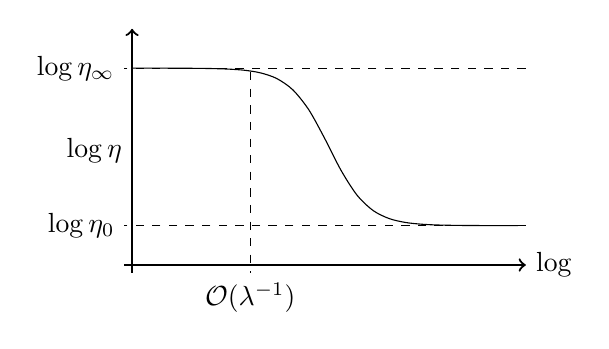
\begin{tikzpicture}
		\draw[thick,->] (-0.1, 0) -- (5,0) node[right] {$\log \srate$};
		\draw[thick,->] (0,-0.1) -- (0, 3) node[left,midway] {$\log \eta$};
		\draw[smooth,domain=0:4.9] plot({\x},{2/(1+exp(4*\x-10))+0.5});		
		\draw[dashed] (5,0.5) -- (-0.1,0.5) node[left] {$\log \eta_0$};
		\draw[dashed] (5,2.5) -- (-0.1, 2.5) node[left] {$\log \eta_\infty$};
		\draw[dashed] (1.5,2.45) -- (1.5,-0.1) node[below] {$\mathcal{O}(\lambda^{-1})$};
	\end{tikzpicture}
\end{center}

\subsubsection{Powell-Eyring \& Ellis models}
The Powell-Eyring model is given by
\begin{equation}
	\frac{\eta(\srate)-\eta_\infty}{\eta_0 - \eta_\infty} =
	\frac{\sinh^{-1}(\lambda \srate)}{\lambda \srate}
\end{equation}

Some models specify $\eta(\sigma)$ instead of $\eta(\srate)$, for example the
Ellis model.
\begin{equation}
	\eta = \eta_0 \left[ 1 + \abs{\frac{\sigma}{\sigma_0}}^{1-n}\right]^{-1}
\end{equation}

There are several properties and issues associated with generalised Newtonian
fluids.
\begin{enumerate}
	\item Empirical: GNFs are based on experiments rather than derived.
	\item Instantaneous: GNFs have no memory (recall the step shear
		experiment), so are not suitable for modelling unsteady flows. This
		also means GNFs are instantaneously reversible which is undesired.
	\item No normal stress differences.
	\item Under extension, the Troutou ratio is $\text{Tr} = 3$ for GNFs, i.e.
		there is no increase in extensional viscosity.

	\item The behaviour of stress when $\srate \to 0$ is important. If
		$\eta_0$ can be defined, then $\sigma \to 0$. If not, such as with a
		power-law fluid, there is problematic behavoiur near $0$. The limit
		$\srate \to 0$ is often used to recover Newtonian behaviour.
\end{enumerate}

\subsection{Rheometry}
\emph{Rheometry} is the science and engineering of measuring material
properties of fluids. For generalised Newtonian fluids, we need to measure
$\eta(\srate)$. The `easy' method is to use a steady shear flow, which is
simple in principle. However, we can only use a finite volume of fluid. A
common solution is the \emph{parallel plate rheometer}, also known as a
parallel disc rheometer. 

Consider two coaxial rigid circular discs of radius $a$ held at a constant separation
$h$. The bottom plate is held stationary whilst the upper plate rotates at a
prescribed angular velocity $\Omega$. The variable $\srate$ is controlled in
this experiment.

\begin{center}
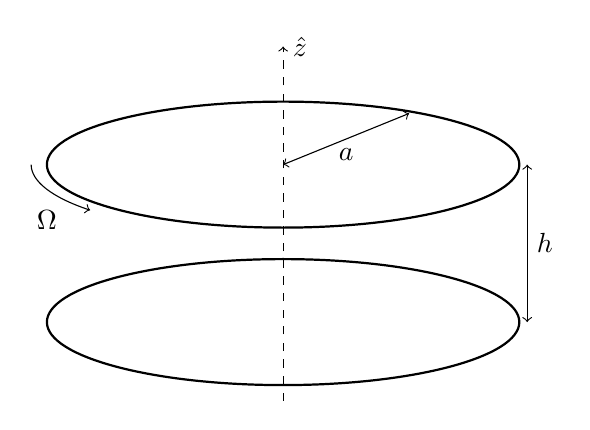
\begin{tikzpicture}
	\draw[thick] (0,0) ellipse (3 and 0.8);
	\draw[thick] (0,-2) ellipse (3 and 0.8);
	\draw[dashed, ->] (0,-3) -- (0,1.5) node[right] {$\hat{\symbf{z}}$};
	\draw[<->] (0,0) -- (1.6,0.65) node[midway,below] {$a$};
	\draw[<->] (3.1, 0) -- (3.1, -2) node[midway,right] {$h$};
	\draw[->] (0, 0) [partial ellipse = -180:-140:3.2 and
	0.9];
	\draw (-3, -0.7) node {$\Omega$};
\end{tikzpicture}
\end{center}

The input-output relationship can be inverted to infer $\eta(\srate)$. Use
cylindrical coordinates $(r, \theta, z)$ and look for an axisymmetric flow
field $\symbf{u} = u(r,z) \hat{\symbf{\theta}}$. The shear rate tensor is
\begin{equation}
	\symbfsf{\srate} = \begin{pmatrix} 0 & r\frac{\partial}{\partial r} \left(
		\frac{u}{r}\right) & 0 \\ r\frac{\partial}{\partial r} \left(
	\frac{u}{r}\right) & 0 & \frac{\partial u}{\partial z} \\
0 & \frac{\partial u}{\partial z} & 0 \end{pmatrix}
\end{equation}

Consider the steady Cauchy equation in cylindrical coordinates:
\begin{align}
	\frac{\partial p}{\partial \theta} &= 0 = \frac{1}{r^2} \frac{\partial
		}{\partial r} \left( r^2 \tau_{r\theta}\right) + \frac{\partial}{\partial
z}\left( \tau_{\theta z}\right) \\
\frac{\partial p}{\partial r} &= 0 \\ \frac{\partial p}{\partial z} &= 0
\end{align}


We wish to find a viscometric flow solution. In the Newtonian case, we have
\begin{equation}
	0 = \frac{1}{r^2} \frac{\partial
		}{\partial r} \left( r^3 \frac{\partial}{\partial r} \left(
	\frac{u}{r}\right)\right) + \frac{\partial^2 u}{\partial z^2}\\
\end{equation}

To find a solution we require both terms vanish. Thus $u = A(r) z + B(r)$. The
no-slip boundary condition $u = 0$ at $z=0$ and $u = \Omega r$ at $z = h$
gives
\begin{equation}
	u(r,z) = \Omega r \frac{z}{h}
\end{equation}

Given this flow, the shear rate tensor becomes
\begin{equation}
	\symbfsf{\srate} = \begin{pmatrix} 0 & 0 & 0 \\ 
		0 & 0 & \frac{r \Omega}{h} \\
0 & \frac{r \Omega}{h} & 0 \end{pmatrix}
\end{equation}

Assume $\Omega > 0$, so the magnitude of the shear rate is $\srate =
\abs{r\Omega/h}$. This solution is also a solution for a GNF: we have
$\tau_{r\theta} = 0$ and 
\begin{equation}
	\tau_{\theta z} = \eta(\srate) \srate =
	\eta(\frac{r\Omega}{h})\frac{r\Omega}{h} = \tau_{\theta z} (r)
\end{equation}

The torque exerted to rotate the top plate is $\symbf{T} = T\hat{\symbf{z}}$ where
\begin{equation}
	T = \int r \tau_{\theta z} \, \diffd S = 2\pi \int_0^a r^2 \eta(\srate)
	\srate \, \diffd r
\end{equation}

This relationship can be used to infer $\eta(\srate)$ by a change of variable.
Let $\srate_a = a\Omega/h$ be the shear rate at the edge of the disc.
Substitute $r = a \srate/\srate_a$:
\begin{equation}
	T = 2\pi \int_0^{\srate_a} \frac{a^2}{\srate_a^2} \srate^2
	\eta(\srate)\srate \frac{a}{\srate_a} \, \diffd \srate = 2\pi
	\frac{a^3}{\srate_a^3} \int_0^{\srate_a} \eta(\srate) \srate^3 \, \diffd
	\srate
\end{equation}
This is valid for all values of $\srate_a$. Rearranging and differentiating
with respect to $\srate_a$ we have
\begin{equation}
	\eta(\srate_a) = \frac{1}{\srate_a^3} \frac{\diffd}{\diffd \srate^a}
	\left[ \frac{T \srate_a^3}{2\pi a^3}\right]
\end{equation}

In an experiment, we control $\srate_a$, measure $T$, slightly change
$\srate_a$, and repeat. Application of the above result then yields
$\eta(\srate_a)$. Other geometries can also be used:
\begin{itemize}
	\item Taylor-Couette.
		\begin{center}
			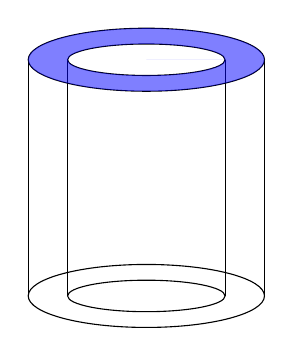
\begin{tikzpicture}
				\draw[name path =A] (0,0) ellipse (1 and 0.2);
				\draw[name path =B] (0,0) ellipse (1.5 and 0.4);
				\draw (0,-3) ellipse (1 and 0.2);
				\draw (0,-3) ellipse (1.5 and 0.4);
				\draw (1.5,0) -- (1.5, -3);
				\draw (-1.5, 0) -- (-1.5, -3);
				\draw (1, 0) -- (1, -3);
				\draw (-1, 0) -- (-1, -3);
				\tikzfillbetween[of=A and B]{blue, opacity=0.5}
			\end{tikzpicture}
		\end{center}
	\item Cone and plate. Useful since $\alpha$ small implies the shear rate
		$\srate$ is uniform.
		\begin{center}
			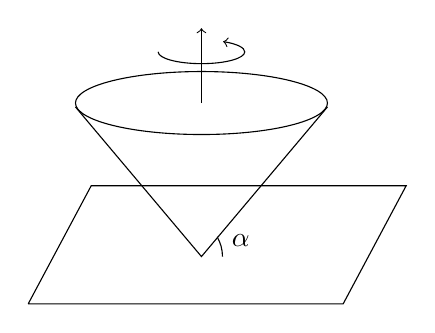
\begin{tikzpicture}
				\draw (-2,0) -- (2,0) -- (2.8, 1.5) -- (-1.2, 1.5) -- (-2,0);
				\draw (-1.4, 2.5) -- (0.2, 0.6) -- (1.8, 2.5);
				\draw (0.2, 2.55) ellipse (1.6 and 0.4);
				\draw (0.4, 0.85) arc (30:0:0.5);
				\draw (0.7, 0.8) node {$\alpha$};
				\draw[->] (0.2, 2.55) -- (0.2, 3.5);
				\draw[->] (0.2, 3.2) [partial ellipse = -180:60:0.55 and
				0.15];
			\end{tikzpicture}
		\end{center}
\end{itemize}

\lecture{22/10/20}
\subsection{Variational approach}
So far, we have found exact solutions only. For many GNF, no exact solutions
are available so we must find approximate solutions. Here we consider a method
relying on a form of energy minimisation. Conider a fluid volume V, bounded by
a surface S, in the Stokes flow limit (no inertia). Assume $\symbf{u} = \symbf{u}_0$
is prescribed on $S$. The total rate of energy dissipation is
\begin{equation}
	P = \int_V \frac{1}{2}\symbfsf{\sigma}:\symbfsf{\srate}\,\diffd V = \int_V
	\frac{\eta}{2} \symbfsf{\srate}:\symbfsf{\srate} \, \diffd V \ge 0
\end{equation}

Recall the minimum dissipation theorem: solutions to Stokes equations minimise
$P$ over all incompressible flows satisfying the same boundary conditions. The
inequality $P_{\text{Stokes}} \le P$ can be shown directly, or we can use the
calculus of variations. Define a Lagrangian
\begin{equation}
	\mathcal{L} \equiv P + \int_V \lambda \nabla \cdot \symbf{u} \, \diffd V
\end{equation}

Variations with respect to $\lambda$ give $\nabla \cdot \symbf{u} = 0$, and
variations with respect to $\symbf{u}$ give Stokes equations with pressure $p
\propto \lambda$. To generalise this to GNF, consider the power density $f =
\frac{1}{2}\eta \srate^2$ for a Newtonian fluid. Analogously, for a GNF we define
\begin{equation}
	f = \int_0^{\srate} \eta(x)x\, \diffd x
\end{equation}
and a new Lagrangian
\begin{equation}
	\mathcal{L} \equiv \mathcal{L}\left[\symbf{u},\lambda\right] = \int_V f \, \diffd
	V + \int_V \lambda \nabla \cdot \symbf{u}\,\diffd V
\end{equation}

\subsubsection{Calculus of variations}
Consider a functional $J$ of a vector field $\symbf{y}(\symbf{x})$ and its
spatial derivatives $y_{m,n} \equiv \frac{\partial y_m}{\partial x_n}$;
\begin{equation}
	J\left[\symbf{y}\right] = \int_V F(x_i,y_j,y_{m,n}) \, \diffd V
\end{equation}
where $V$ is the total domain. The \emph{first variation} of $J$ is $\delta J$ where
\begin{equation}
	J + \delta J = J\left[\symbf{y}+\delta\symbf{y}\right] = \int_V
	F(\symbf{x},\symbf{y}+\delta\symbf{y})\,\diffd V
\end{equation}
To determine an explicit expression for the first variation, first Taylor
expand the integrand:
\begin{equation}
	F(\symbf{x},\symbf{y}+\delta\symbf{y}) = F + \delta y_j \frac{\partial F}{\partial
		y_j} + \delta y_{m,n} \frac{\partial F}{\partial y_{m,n}} + \dots
\end{equation}
Using integration by parts and writing $\delta y_{m,n} =
\frac{\partial}{\partial x_n} \delta y_m$ we have
\begin{equation}
	\delta y_{m,n} \frac{\partial F}{\partial y_{m,n}} = 
	\frac{\partial}{\partial x_n}\left( \delta y_m \frac{\partial F}{\partial
		y_{m,n}}\right) - \delta y_m \frac{\partial}{\partial x_n} \left(
	\frac{\partial F}{\partial y_{m,n}}\right)
\end{equation}

The first term becomes a surface integral via Stokes' theorem, which may or
may not vanish depending on boundary conditions. The first variation of $F$ is
thus
\begin{equation}
	\delta F = \delta y_j \left[ \frac{\partial F}{\partial y_j} -
		\frac{\partial}{\partial x_n} \left( \frac{\partial F}{\partial
	y_{j,n}}\right)\right] + \text{boundary terms}
\end{equation}

Now requiring $\delta J = 0$ for all $\delta y$ is equivalent to requiring
$\delta F = 0$ for all $\delta y$, giving the \emph{Euler-Lagrange equation}.
\begin{equation}
\frac{\partial F}{\partial y_j} - \frac{\partial}{\partial x_n} \left(
\frac{\partial F}{\partial y_{j,n}}\right) = 0
\end{equation}

\subsubsection{Variational solution}
Returning to our original set-up, denote $F_2 = \lambda \nabla \cdot \symbf{u}$,
$F_1 = \int_0^{\srate} \eta(x)x\,\diffd x$, so
\begin{equation}
	\mathcal{L}\left[\symbf{u},\lambda\right] = \int_V F_1 + F_2\,\diffd V
\end{equation}

Note that we are using $\symbf{y} \equiv \symbf{u}$ here.  The Euler-Lagrange
equation for $\lambda $ gives
\begin{equation}
	\frac{\partial}{\partial \lambda} \left( F_1 + F_2\right) = 0 \implies
	\nabla \cdot \symbf{u} = 0
\end{equation}

For variations with respect to $\symbf{u}$, we have boundary terms involving
$\delta \symbf{u}$. Since $\delta \symbf{u} = \symbf{0}$ on $S$, the boundary terms
vanish in this case. There is no explicit dependence on $\symbf{u}$ in $F_1, F_2$
so the Euler-Lagrange equation becomes
\begin{equation}
	\frac{\partial}{\partial x_n} \left( \frac{\partial F}{\partial
	u_{j,n}}\right) = 0
\end{equation}

where $F \equiv F_1 + F_2$. By chain rule, 
\begin{equation}
	\frac{\partial F_1}{\partial u_{j,n}} = \frac{\partial \srate}{\partial
	u_{j,n}} \frac{\partial F_1}{\partial \srate}
\end{equation}
We have $\frac{\partial F_1}{\partial \srate} = \eta(\srate) \srate$ and
\begin{align}
	\frac{\partial \srate}{\partial u_{j,n}} &=
	\frac{1}{2\srate} \frac{\partial}{\partial u_{j,n}} \left( \frac{1}{2}
	\symbfsf{\srate}:\symbfsf{\srate}\right) \\
	&= \frac{1}{2\srate} \frac{\partial}{\partial u_{j,n}} \left( \frac{1}{2}
	\srate_{pq} \srate_{pq}\right) \\
	&= \frac{1}{4\srate} \frac{\partial}{\partial u_{j,n}}\left(
u_{p,q}u_{p,q} + 2u_{p,q}u_{q,p} + u_{q,p}u_{q,p}\right) \\
&= \frac{1}{2\srate} \left( 2 u_{j,n} + 2u_{n,j}\right) \\
&= \frac{\srate_{jn}}{\srate}
\end{align}

Now for $F_2 = \lambda \nabla \cdot \symbf{u}$ we have
\begin{align}
	\frac{\partial}{\partial x_n} \left( \frac{\partial F_2}{\partial u_{j,n}}
		\right) &= \frac{\partial}{\partial x_n} \left( \lambda
		\frac{\partial u_{i,i}}{\partial u_{j,n}}
	\right) \\
	&= \frac{\partial}{\partial x_n} \left( \lambda \delta_{ij}
\delta_{in}\right) \\
&= \frac{\partial \lambda}{\partial x_j}
\end{align}

Thus the full Euler-Lagrange equation for $\symbf{u}$ is
\begin{equation}
	\frac{\partial}{\partial x_n} \left[ \eta(\srate) \srate_{jn}\right] +
	\frac{\partial \lambda}{\partial x_j} = 0
\end{equation}
for $j= 1, 2, 3$. Given $\lambda = -p$, this becomes the Cauchy equation for a
GNF.
\begin{equation}
	-\nabla p + \nabla \cdot \left[ \eta(\srate) \symbfsf{\srate}\right] =
	\symbf{0}
\end{equation}

Pressure is used as a Lagrange multiplier to enforce incompressibility. Note:
if the boundary conditions are different, e.g. $\symbfsf{\sigma} \cdot \symbf{n}$
is prescribed, we must distinguish surfaces where $\symbf{u}$ is described and
surfaces where $\symbfsf{\sigma} \cdot \symbf{n}$ is prescribed, and add a surface
integral to the Lagrangian (see Example Sheet 1).

To generate approximate solutions to the Cauchy GNF equations, we note that
the closer the value of $\mathcal{L}$ to its minimum, the better the
approximation. Thus
\begin{enumerate}
	\item Use incompressible test functions $\symbf{u}_\alpha$ where $\alpha$ is
		a parameter
	\item Substitute into Lagrangian, minimise with respect to $\alpha$
	\item If the minimum of $\mathcal{L}$ is at $\alpha = \alpha^*$ then
		$\symbf{u}_{\alpha^*}$ is an approximate solution
\end{enumerate}

Integrals involved in $\mathcal{L}$ in general have to be evaluated
numerically. Choice of test functions comes from physical intuition,
computation, or experiment.

\lecture{27/10/20}
\section{Yield-Stress Fluids}
Some fluids only flow when subject to stress above some threshold. We call
this threshold the \emph{yield-stress}, denoted by $\sigma_y$. Fluids with such
a property are called \emph{yield-stress fluids} or \emph{viscoplastic fluids}.
Examples are mayonnaise; jelly; peanut butter; mud; and hair gel. Graphically,
$\sigma_y$ is the non-zero $\srate$-intercept of $\sigma(\srate)$. Beyond the
yield-stress, the fluid may have Newtonian, shear-thinning, shear-thickening,
or some other behaviour. 

The simplest model of a yield-stress fluid is a \emph{Bingham fluid} where the
behaviour is Newtonian beyond the yield-stress. For $-\infty < \srate <
\infty$ we have
\begin{equation}
	\begin{cases}
		\srate = 0 & \abs{\sigma} < \sigma_y \\
		\sigma = \text{sgn}(\srate)\sigma_y + \eta \srate & \abs{\sigma} > \sigma_y
	\end{cases}
\end{equation}

Alternatively, non-linear behaviour after yield is described by the
\emph{Herschel-Bulkley model} where the fluid has power-law behaviour after
yield. 
\begin{equation}
	\begin{cases}
		\srate = 0 & \abs{\sigma} < \sigma_y \\
		\sigma = \text{sgn}(\srate)\sigma_y + \kappa \abs{\srate}^{n-1} \srate
		& \abs{\sigma} > \sigma_y 
	\end{cases}
\end{equation}

\begin{center}
	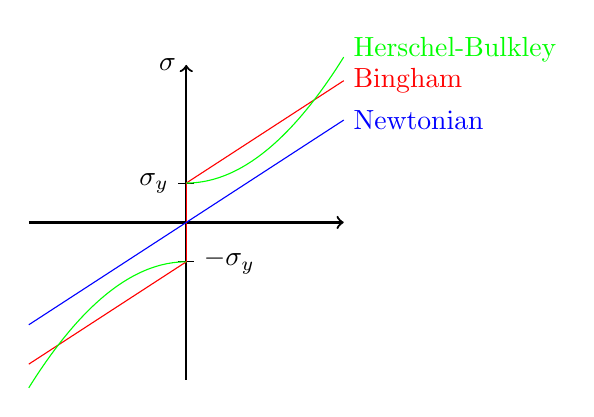
\begin{tikzpicture}
		\draw[thick,->] (-2, 0) -- (2,0) node[right] {$\srate$};
		\draw[thick,->] (0,-2) -- (0, 2) node[left] {$\sigma$};
		\draw (0.1, 0.5) -- (-0.1, 0.5) node[left] {$\sigma_y$};
		\draw (-0.1, -0.5) -- (0.1, -0.5) node[right] {$-\sigma_y$};
		\draw[red] (0, -0.5) -- (0, 0.5);
		\draw[red] (0, 0.5) -- (2, 1.8) node[right] {Bingham};
		\draw[red] (0, -0.5) -- (-2, -1.8);
		\draw[blue] (-2,-1.3) -- (2,1.3) node[right] {Newtonian};
		\draw[green, smooth] plot[domain=0:2] ({\x},{0.5+0.4*\x*\x});
		\draw[green, smooth] plot[domain=-2:0] ({\x},{-0.5-0.4*\x*\x});
		\draw[green] (2,2.2) node[right] {Herschel-Bulkley};
	\end{tikzpicture}
\end{center}

A typical flow problem of yield-stress fluids separates the domain into two
regions.
\begin{enumerate}
	\item Yielded domain: the fluid flows in regions where $\abs{\sigma} >
		\sigma_y$
	\item Unyielded domain: where $\abs{\sigma} < \sigma_y$, there is no
		deformation i.e. rigid body motion only
\end{enumerate}

The surface separating the yielded and unyielded regions is the \emph{yield
surface}. On this surface, $\sigma = \sigma_y$ by definition, which implicitly
defines the surface. Physically, we expect high shear at boundaries, and thus
expect the yield surface is close to these boundaries.

\subsection{Pressure-driven flow of a Bingham fluid in a pipe}
This problem illustrates a steady flow problem and the location of the yield
surface. We will use cylindrical coordinates, and assume the flow is
unidirectional with $\symbf{u} = u(r) \hat{\symbf{z}}$.

\begin{center}
\begin{tikzpicture}
	\draw (0,0) ellipse (0.6 and 1);
	\draw (0,-1) -- (8,-1);
	\draw (0, 1) -- (8,1);
	\draw (8,0) [partial ellipse = -90:90:0.6 and
	1];
	\draw[dashed] (8,0) [partial ellipse = 90:270:0.6 and
	1];
	\draw[thick,blue,->] (4,0) -- (6, 0) node[right] {flow};
	\draw (-2, 0) node {$p_0 + \Delta p$};
	\draw (10, 0) node {$p_0$};
	\draw[->] (0,0) -- (0,1) node[midway,right] {$R$};
	\draw[<->] (0,-1.5) -- (8,-1.5) node[midway, below] {$L$};
\end{tikzpicture}
\end{center}

The Cauchy equation in cylindrical polars (as seen in section~\ref{sec:pipe})
gives
\begin{equation}
	\frac{\partial p}{\partial z} = \frac{1}{r} \frac{\partial}{\partial r}
	\left( r \sigma_{rz} \right) = -\frac{\Delta p}{L}
\end{equation}
thus as before we find
\begin{equation}
	\sigma_{rz} = -\frac{\Delta p}{2L} r
\end{equation}
We wish to find the yield surface. Clearly near $r=0$ the stress is small
so the fluid is unyielded. The yield surface is defined by $\abs{\sigma} =
\sigma_y$ thus we have
\begin{equation}
	r = r_y = \frac{2L}{\Delta p} \sigma_y
\end{equation}
Recall $R$ is the radius of the pipe. Comparing $R$ with $r_y$,
\begin{enumerate}
	\item if $r_y \ge R$ the shear stress is below yield stress thoughout the
		pipe, thus there is no flow. Equivalently, this occurs for pressure
		differences $\Delta p \le \frac{2L}{R} \sigma_y$.
	\item if $r_y < R$ (equivalently $\Delta p > \frac{2L}{R} \sigma_y$) the
		fluid yields in $r_y \le r \le R$, and is unyielded in $0 \le r \le
		r_y$.
\end{enumerate}

We solve case 2 exactly. Flow in the yielded region has $\srate =
\frac{\partial u}{\partial r} < 0$. For a Bingham fluid $\sigma =
\text{sgn}(\srate) \sigma_y + \eta \srate$. Therefore we have
\begin{equation}
	\sigma_{rz} = -\sigma_y + \eta \frac{\partial u}{\partial r}
\end{equation}
Now $\sigma_{rz} = -\frac{\Delta p}{2L} r$ can be rewritten in terms of the
yield surface as $\sigma_{rz} = -\sigma_y \frac{r}{r_y}$. Thus we must solve
\begin{equation}
	\frac{\partial u}{\partial r} = \frac{\sigma_y}{\eta}\left( 1 -
	\frac{r}{r_y}\right)
\end{equation}
Note $r = r_y$ implies $\frac{\partial u}{\partial r} = 0$ which gives
$\abs{\sigma} = \sigma_y$ as expected. We have
\begin{equation}
u(r) = \frac{\sigma_y}{\eta} \left(r - \frac{r^2}{2r_y}\right) + c
\end{equation}
The constant of integration is determined by the no-slip boundary condition on
$r=R$, $u(R) = 0$. Finally we have for $r_y \le r \le R$
\begin{equation}
	u(r) = \frac{\sigma_y}{\eta} \left( r - \frac{r^2}{2r_y} - R +
	\frac{R^2}{2r_y}\right)
\end{equation}

In the unyielded region we have plug flow $u =$ constant.  For $0 \le r \le
r_y$, the rigid body velocity $u = U_y = u_{\text{yielded}}(r_y)$ by
continuity.
\begin{equation}
	\implies U_y = \frac{\sigma_y}{\eta} \left( \frac{r_y}{2} - R +
	\frac{R^2}{2r_y}\right) \ge 0
\end{equation}

The flow profile in the pipe is a combination of parabolic and constant
velocity.
\begin{center}
	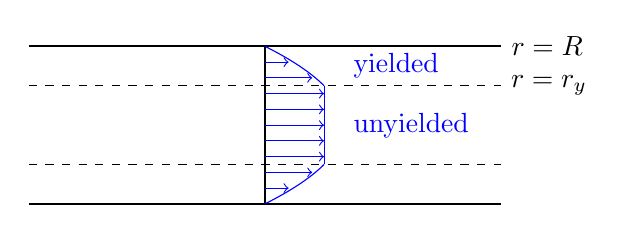
\begin{tikzpicture}
		\draw[thick] (-3, 1) -- (3, 1) node[right] {$r=R$};
		\draw[thick] (-3, -1) -- (3, -1);
		\draw (0, 1) -- (0, -1);
		\draw[dashed] (-3, 0.5) -- (3, 0.5) node[right] {$r=r_y$};
		\draw[dashed] (-3, -0.5) -- (3, -0.5);
		\draw[smooth,blue,domain=-1:-0.5,variable=\y] plot({1-\y*\y},{\y});
		\draw[smooth,blue,domain=1:0.5,variable=\y] plot({1-\y*\y},{\y});
		\draw[blue] (0.75, 0.5) -- (0.75, -0.5);
		\draw (1, 0) node[blue,right] {unyielded};
		\draw (1, 0.75) node[blue,right] {yielded};
		\draw[blue,->] (0,0.4) -- (0.75, 0.4);
		\draw[blue,->] (0,0.2) -- (0.75, 0.2);
		\draw[blue,->] (0,0) -- (0.75,0);
		\draw[blue,->] (0,-0.4) -- (0.75, -0.4);
		\draw[blue,->] (0,-0.2) -- (0.75, -0.2);
		\draw[blue,->] (0,0.6) -- (0.6, 0.6);
		\draw[blue,->] (0,0.8) -- (0.3, 0.8);
		\draw[blue,->] (0,-0.6) -- (0.6, -0.6);
		\draw[blue,->] (0,-0.8) -- (0.3, -0.8);
	\end{tikzpicture}
\end{center}

The flow rate $Q$ vanishes if $r_y \ge R$. For $r_y < R$, 
\begin{align}
	Q &= 2\pi \int_0^R r u(r) \, \diffd r \\
	  &= 2\pi \int_0^{r_y} rU_y \, \diffd r + 2\pi \int_{r_y}^R ru(r) \,
	\diffd r \\
	&= \dots \\
	&= \frac{\Delta p \pi R^4}{8\mu L} \left[ 1 - \frac{4}{3}\frac{r_y}{R} +
	\frac{1}{3} \left( \frac{r_y}{R}\right)^3\right]
\end{align}

The constant factor outside the brackets is the \emph{Hagen-Poiseuille flow
rate} for a Newtonian fluid.
\begin{itemize}
	\item If $r_y = 0$ the fluid is yielded everywhere and we have the
		Newtonian solution for Poiseuille flow in a pipe.
	\item If $r_y = R$ the fluid is unyielded everywhere and $Q = 0$.
	\item The term in brackets is always smaller than $1$, thus
		$Q_{\text{yield-stress}} \le Q_{\text{Newtonian}}$
\end{itemize}

This problem is doable because it is a steady problem. It is much more
difficult in the unsteady case since the yield surface has unsteady motion, in
which case inertia is needed.

\lecture{29/10/20}
\subsection{Unsteady dynamics of yield surface}
Here we include inertia to allow the yield surface to go from one steady state
to another. Specifically, we consider a problem similar to Stokes' 1st
problem, to illustrate the complexity of solving for the yield surface. In
Stokes' 1st problem, a rigid plate at $y=0$ impulsively starts to move at
$t=0$. The momentum `diffuses' into the fluid as $y \sim \sqrt{\nu t}$.

Consider a Bingham fluid in $y > 0$ with yield stress $\sigma_y$, viscosity
$\eta$, density $\rho$ and a rigid plate at $y=0$. For $t < 0$, we have a
semi-infinite shear flow $\symbf{u} = \srate y \hat{\symbf{x}}$. Note: we require
$\sigma = \eta \srate > \sigma_y$ to ensure there is flow everywhere. At
$t=0$, the plate starts to move with the flow such that the stress exerted on
the plate suddenly changes to $\sigma_0 < \sigma_y$. 

\begin{center}
	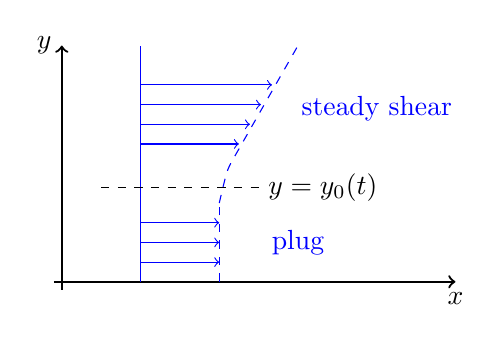
\begin{tikzpicture}
		\draw[thick,->] (-0.1, 0) -- (5, 0) node[below] {$x$};
		\draw[thick,->] (0,-0.1) -- (0, 3) node[left] {$y$};
		\draw[blue] (1,0) -- (1,3);
		\draw[dashed,blue] (2,0) -- (2, 1);
		\draw[dashed,blue] (2.2,1.6) -- (3,3);
		\draw[dashed,blue] plot [smooth] coordinates {(2,1) (2.1, 1.4)
		(2.2,1.6)};
		\draw[dashed] (0.5,1.2) -- (2.5,1.2) node[right] {$y=y_0(t)$};
		\draw[blue] (3, 0.5) node {plug};
		\draw[blue] (4, 2.2) node {steady shear};
		\draw[blue,->] (1,0.25) -- (2, 0.25);
		\draw[blue,->] (1,0.5) -- (2, 0.5);
		\draw[blue,->] (1,0.75) -- (2, 0.75);
		\draw[blue,->] (1,1.75) -- (2.25,1.75);
		\draw[blue,->] (1,2) -- (2.39,2);
		\draw[blue,->] (1,2.25) -- (2.53,2.25);
		\draw[blue,->] (1,2.5) -- (2.67,2.5);
	\end{tikzpicture}
\end{center}

Physically, the unyielded domain appears near $y=0$ and propagates into the
yielded region. Let $y=y_0(t)$ be the yielded surface, so that $0 \le y \le
y_0$ is the unyielded region region and $y > y_0$ is the unyielded region. On
the yield surface, we require $\abs{\sigma} = \sigma_y$ by definition, and
also require the velocity to be continuous across the yield surface.

Assuming the flow is unidirectional with $\symbf{u} = u(y,t)\hat{\symbf{x}}$, the Cauchy
equation with inertia is valid in both the yielded and unyielded domain:
\begin{equation}
	\rho \frac{\partial u}{\partial t} = \frac{\partial \sigma}{\partial y}
\end{equation}

\paragraph{Yielded region.} We have $\sigma = \sigma_{xy} = \sigma_y + \eta
\frac{\partial u}{\partial y}$, since $\srate = \frac{\partial u}{\partial y}
\ge 0$. Thus the Cauchy equation becomes
\begin{equation}
	\frac{\partial u}{\partial t} = \nu \frac{\partial^2 u}{\partial y^2}
\end{equation}
where $\nu = \eta/\rho$ is the kinematic viscosity. This is a diffusion
equation; as in Stokes' 1st problem, the yield surface has diffusive dynamics
$y_0 \sim \sqrt{\nu t}$. Look for a similarity solution with dimensionless
variable $s \equiv \frac{y}{\sqrt{\nu t}}$. Then
\begin{align}
	u(y,t) &= \srate y f(s)\\
	\frac{\partial u}{\partial t} &= -\frac{1}{2}\frac{s}{t} \srate y
	\frac{\diffd f}{\diffd s} \\
	\frac{\partial u}{\partial y} &= \srate f + \srate s \frac{\diffd
	f}{\diffd s} \\
	\frac{\partial^2 u}{\partial y^2} = 2 \frac{\srate s}{y} \frac{\diffd
	f}{\diffd s} + \srate \frac{s^2}{y}\frac{\diffd^2 f}{\diffd s^2}
\end{align}

The Cauchy equation is now
\begin{equation}
	-\frac{1}{2}\frac{s}{t}\srate y \frac{\diffd f}{\diffd s} = \nu \left[ 2
		\frac{\srate s}{y} \frac{\diffd f}{\diffd s} + \frac{\srate s^2}{y}
	\frac{\diffd^2 f}{\diffd s^2} \right] 
\end{equation}
Dividing by $\nu \srate s/ y$ and rearranging we have the ODE
\begin{equation}
	\left( 2+ \frac{s^2}{2}\right) \frac{\diffd f}{\diffd s} + \frac{\diffd^2
	f}{\diffd s^2} = 0
\end{equation}

Since the ODE is second order, we require two boundary conditions:
\begin{enumerate}
	\item Match steady shear as $y \to \infty$, i.e. $f(s) \to 1$.
	\item At yield surface, $\sigma(y_0^+) = \sigma(y_0^-) = \sigma_y$.
		Equivalently, $u_y = 0$ at $y = y_0$. Thus we require
		\begin{equation}
			\srate f + \srate s \frac{\diffd f}{\diffd s } = 0
		\end{equation}
		at $y = y_0$. Writing the location of the yield surface as $y_0 =
		\theta \sqrt{\nu t}$ with $\theta$ unknown we have
		\begin{equation}
			f(\theta) + \theta f'(\theta) = 0
		\end{equation}
\end{enumerate}

\paragraph{Unyielded region.} The same Cauchy equation holds, $\rho \partial_t
u = \partial_y \sigma$. The flow in this region is a plug, so $u$ does not
depend on $y$. Thus $\partial_y \sigma$ is constant, i.e. $\sigma$ is linear
in $y$ in this region. Now note at $y=y_0, \sigma=\sigma_y$ and at $y=0,
\sigma=\sigma_0$. So
\begin{equation}
	\frac{\partial \sigma}{\partial y} = \frac{\sigma_y - \sigma_0}{y_0} =
		\frac{\sigma_y - \sigma_0}{\theta \sqrt{\nu t}}
\end{equation}

Thus the Cauchy equation becomes
\begin{equation}
	\rho \frac{\partial u}{\partial t} = \frac{\sigma_y - \sigma_0}{\theta
	\sqrt{\nu t}}
\end{equation}
Integrating from $t' = 0$ to $t' = t$, we have
\begin{equation}
	\rho u_{\text{unyielded}} = 2 \frac{\sigma_y - \sigma_0}{\theta \nu^{1/2}}
	t^{1/2}
\end{equation}
Note $u_{\text{unyielded}} = u_{\text{yielded}}(y_0) = \srate y_0 f(\theta) =
\srate \theta \sqrt{\nu t} f(\theta)$, so
\begin{align}
	\rho \srate \theta \sqrt{\nu t} f(\theta) &= 2 \frac{\sigma_y -
	\sigma_0}{\theta \nu^{1/2}}t^{1/2}\\
	\implies \theta^2 f(\theta) &= 2 \xi
\end{align}
where $\xi = \frac{\sigma_y - \sigma_0}{\eta \srate}$ is a dimensionless
control parameter, i.e. it is imposed on the system. This equation implicitly
defines $\theta$.

\paragraph{Yield surface.}
Now the ODE for $f$ gives
\begin{equation}
	\frac{\diffd f}{\diffd s} = \frac{B}{s^2} e^{-\frac{s^2}{4}}
\end{equation}
Integrating and using $f(s \to \infty) = 1$ we have
\begin{equation}
	f(s) = 1 + \frac{C}{s} e^{-s^2/4} - \frac{\sqrt{\pi}}{2}C
	\text{erfc}(s/2)
\end{equation}
where $\text{erfc}(x) \equiv \frac{2}{\sqrt{\pi}} \int_x^\infty e^{-u^2} \,
\diffd u$ is the \emph{complementary error function}. To determine $C$, we
apply the BC $u_y = 0$ at the yield surface, i.e. $f(\theta) + \theta
f'(\theta) = 0$
\begin{align}
	\implies C &= \frac{2}{\sqrt{\pi} \text{erfc}(\theta/2)} \\
	\implies f(s) &= 1 + \frac{\frac{2}{s} e^{-s^2/4} -
	\sqrt{\pi}\text{erfc}(s/2)}{\sqrt{\pi} \text{erfc}(\theta/2)}
\end{align}
The only remaining unknown is $\theta$. Applying the condition $\theta^2
f(\theta) = 2\xi$, we have
\begin{equation}
	\frac{\theta e^{-\theta^2/4}}{\sqrt{\pi}\text{erfc}(\theta/2)} = \xi =
	\frac{\sigma_y - \sigma_0}{\eta\srate}
\end{equation}
which is an implicit one-to-one equation for $\theta$, so $\theta$ can be
found numerically. Thus we have a full analytic solution up to an implicit
equation for $\theta$.

\section{Linear Viscoelastic Fluids}
Recall from phenomenology that some complex fluids have stresses which depend
on the history of deformation, i.e. they have memory. Generalised Newtonian
fluids and yield-stress fluids have no such memory. To model complex fluids
with memory, we must incorporate \emph{elasticity}.

\subsection{Viscous vs. elastic}
Consider fluids that have both a viscous \emph{and} elastic response to
deformation. Viscous response means that stress is proportional to rate of
deformation, whilst an elastic response means stress is proportional to
deformation. For example, polymer molecules are sheared and stretched by the
flow, and provide an elastic response.

Recall Newton's experiment. Consider two points marked at the same $x$ on the
top and bottom plate at the same time, and the change in the mark as time
passes. The change in position is $d$, the \emph{shear displacement}.
\begin{center}
	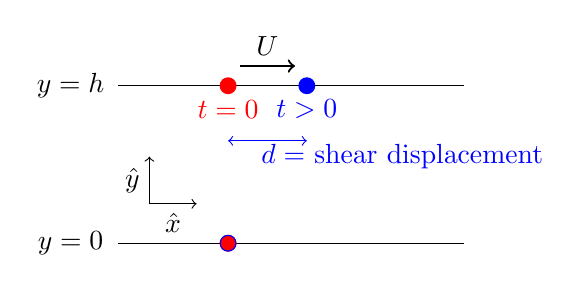
\begin{tikzpicture}
		\node at (0,2) {$y = h$};
		\draw (0.6, 2) -- (5, 2);
		\node at (0,0) {$y=0$};
		\draw (0.6, 0) -- (5,0);
		\node at (2.5, 2.5) {$U$};
		\draw[->, thick] (2.15, 2.25) -- (2.85, 2.25);
		\draw[->] (1,0.5) -- (1.6, 0.5) node[midway,below] {$\hat{\symbf{x}}$};
		\draw[->] (1,0.5) -- (1, 1.1) node[midway, left] {$\hat{\symbf{y}}$};
		\draw[red,fill] (2,0) circle (0.1);
		\draw[red,fill] (2,2) circle (0.1);
		\draw[red] (2,1.7) node {$t=0$};
		\draw[blue,fill] (3,2) circle (0.1);
		\draw[blue] (2,0) circle (0.1);
		\draw[blue] (3,1.7) node {$t>0$};
		\draw[blue,<->] (2,1.3) -- (3,1.3);
		\draw[blue] (2.3, 1.1) node[right] {$d = $ shear displacement};
	\end{tikzpicture}
\end{center}

We then define \emph{shear strain} $\gamma = \frac{d}{h}$, dimensionless, and
as usual have shear rate $\srate = \frac{U}{h} = \frac{\diffd \gamma}{\diffd
t}$. The viscous response (Newtonian) is $\sigma = \frac{F}{A} = \eta \srate$
where $\eta$ is the viscosity. The \emph{elastic} response, in analogy with a
spring $F \propto kx$, we have $\sigma = G \gamma$ where $G$ is the
\emph{shear modulus} and has units of stress.

Physically, a \emph{dashpot} simulates viscous response, whilst a spring
simulates elastic response. The simplest viscoelastic materials can be thought
of as a linear combination of dashpots and springs.

\lecture{3/11/20}
\subsection{Maxwell fluids}
The most famous linear viscoelastic fluid (LVF) is a \emph{Maxwell fluid};
modelled by a dashpot and a spring in \emph{series}. We expect elastic
behaviour on short timescales and viscous on long timescales. An example of a
Maxwell fluid is a fluid with elastic inclusions such as droplets or vesicles.

\begin{center}
	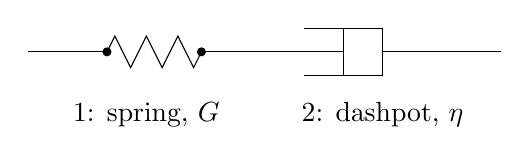
\begin{tikzpicture}
		\draw (-3, 0) -- (-2, 0);
		\draw[fill] (-2, 0) circle (0.05);
		\draw (-2, 0) -- (-1.9, 0.2) -- (-1.7, -0.2) -- (-1.5, 0.2) -- (-1.3,
		-0.2) -- (-1.1, 0.2) -- (-0.9, -0.2) -- (-0.8,0);
		\draw[fill] (-0.8, 0) circle (0.05);
		\draw (-0.8,0) -- (1,0);
		\draw (1,0.3) -- (1, -0.3);
		\draw (0.5, 0.3) -- (1.5, 0.3) -- (1.5, -0.3) -- (0.5, -0.3);
		\draw (1.5, 0) -- (3, 0);
		\draw (-1.5, -0.8) node {1: spring, $G$};
		\draw (1.5, -0.8) node {2: dashpot, $\eta$};
	\end{tikzpicture}
\end{center}

We can derive the constitutive relationship from this model. We have
\begin{align}
	\sigma_1 &= G \gamma_1 \hspace{2em} \text{spring}\\
	\sigma_2 &= \eta \srate_2 \hspace{2em} \text{dashpot} \\
\end{align}

The total stress and strain follow by analogy with circuits (cf. Kirkhoff's
laws). Strain is analogous to potential difference and stress is analogous to
current. Therefore
\begin{align}
	\text{total strain} \hspace{1em}  \gamma &= \gamma_1 + \gamma_2 \\
	\text{total stress}  \hspace{1em} \sigma &= \sigma_1 = \sigma_2
\end{align}

The total rate of strain is 
\begin{align}
	\srate = \srate_1 + \srate_2 &= \frac{\dot{\sigma}_1}{G} +
	\frac{\sigma_2}{\eta} = \frac{\dot{\sigma}}{G} + \frac{\sigma}{\eta}\\ 
	\implies \sigma + \frac{\eta}{G} \dot{\sigma} &= \eta \srate
\end{align}
This is the constitutive relationship for a Maxwell fluid. $\lambda \equiv
\frac{\eta}{G}$ is the \emph{relaxation timescale} for stress.

\paragraph{Intepretation of $\lambda$.} Consider a sudden cessation of
deformation, that is
\begin{equation}
	\begin{cases} \srate = 0 & t \ge 0 \\ \sigma = \sigma_0 & t < 0
	\end{cases}
\end{equation}
Thus for $t > 0$ we have $\sigma + \lambda \dot{\sigma} = 0$ with boundary
conditions $\sigma(t=0) = \sigma_0$. Thus
\begin{equation}
	\sigma(t) = \sigma_0 e^{-\frac{t}{\lambda}}
\end{equation}
Hence we have exponential relaxation of stress on timescale $\lambda$. Note
$\lambda$ is the timescale for adjustments in stress due to changes in
deformation, whilst deformation adjusts instantaneously to changes in stress.

\paragraph{Behaviour at short vs. long timescales.} Consider a Maxwell fluid
for $t \ll \lambda$ and $t \gg \lambda$. 

\begin{itemize}
	\item On short timescales $t \ll \lambda$, we have $\lambda \dot{\sigma}
		\gg \sigma$ hence the Maxwell fluid has $\lambda \dot{\sigma} \sim
		\eta \srate$. This is an elastic response.
	\item On long timescales $t \gg \lambda$, we have $\lambda \dot{\sigma}
		\ll \sigma$ so the Maxwell fluid has $\sigma \sim \eta \srate$ which
		is a viscous response.
\end{itemize}

\subsection{Kelvin-Voigt fluid}
Here we consider a similar idea to introduce a fluid with the opposite
behaviour to a Maxwell fluid. Consider a spring and dashpot in
\emph{parallel}. 

\begin{center}
	\begin{tikzpicture}
		\draw (-3, 0) -- (-1.5, 0);
		\draw[fill] (-1.5, 0) circle (0.05);
		\draw (-1.5, 0) -- (-1.4, 0.2) -- (-1.2, -0.2) -- (-1, 0.2) -- (-0.8,
		-0.2) -- (-0.6, 0.2) -- (-0.4, -0.2) -- (-0.3,0);
		\draw[fill] (-0.3, 0) circle (0.05);
		\draw (-0.3,0) -- (1,0);
		\draw (-3, -2) -- (-1, -2);
		\draw (-1,-1.7) -- (-1, -2.3);
		\draw (-1.5, -1.7) -- (-0.5, -1.7) -- (-0.5, -2.3) -- (-1.5, -2.3);
		\draw (-0.5, -2) -- (1, -2);
		\draw (-1, 0.8) node {1: spring, $G$};
		\draw (-1, -2.8) node {2: dashpot, $\eta$};
		\draw (-5, -1) -- (-3, -1);
		\draw (-3,0) -- (-3, -2);
		\draw (1,0) -- (1, -2);
		\draw (1, -1) -- (3, -1);
	\end{tikzpicture}
\end{center}

We have individual stresses
\begin{align}
	\sigma_1 &= G \gamma_1 \hspace{2em} \text{spring}\\
	\sigma_2 &= \eta \srate_2 \hspace{2em} \text{dashpot} \\
\end{align}
as before. In parallel, the total strain is $\gamma = \gamma_1 + \gamma_2$ and
the total stress is
\begin{equation}
	\sigma = \sigma_1 + \sigma_2 = G\gamma_2 + \eta \srate_2 = G\left[ \gamma
	+ \frac{\eta}{G} \srate\right]
\end{equation}
Hence the constitutive relationship for a Kelvin-Voigt fluid is
\begin{equation}
	\sigma = G \left[ \gamma + \hat{\lambda}\srate\right]
\end{equation}
where $\hat{\lambda}$ is the \emph{retardation timescale}, the timescale for
deformation to adjust to changes in stress. Note: stress adjusts
instantaneously to changes in deformation in this case.
\begin{itemize}
	\item On short timescales, we have $\hat{\lambda} \srate \gg \gamma$ so $\sigma
		\sim G \hat{\lambda} \srate$ is a viscous response.
	\item On long timescales, we have $\hat{\lambda} \srate \ll \gamma$ so
		$\sigma \sim G \gamma$ which is an elastic response.
\end{itemize}

The properties of Kelvin-Voigt fluids are opposite to those of a Maxwell
fluid. Since a Kelvin-Voigt fluid behaves as an elastic material at long
times, it is also referred to as a viscoelastic \emph{material} or
\emph{solid}.

\subsection{Jeffreys fluid}
We wish to construct a LVF that has a viscous response at both \emph{short}
and \emph{long} timescales. Thus we require two distinct timescales. A
Jeffreys fluid has a dashpot and Kelvin-Voigt fluid in series.

\begin{center}
	\begin{tikzpicture}
		\draw (-5, -0.7) -- (-4,-0.7) -- (-4, -1.3) -- (-5, -1.3);
		\draw (-4.5, -0.7) -- (-4.5, -1.3);
		\draw (-6,-1) -- (-4.5, -1);
		\draw (-4.5, -1.8) node {1: dashpot, $\eta_1$};
		\draw (-3, 0) -- (-1.5, 0);
		\draw[fill] (-1.5, 0) circle (0.05);
		\draw (-1.5, 0) -- (-1.4, 0.2) -- (-1.2, -0.2) -- (-1, 0.2) -- (-0.8,
		-0.2) -- (-0.6, 0.2) -- (-0.4, -0.2) -- (-0.3,0);
		\draw[fill] (-0.3, 0) circle (0.05);
		\draw (-0.3,0) -- (1,0);
		\draw (-3, -2) -- (-1, -2);
		\draw (-1,-1.7) -- (-1, -2.3);
		\draw (-1.5, -1.7) -- (-0.5, -1.7) -- (-0.5, -2.3) -- (-1.5, -2.3);
		\draw (-0.5, -2) -- (1, -2);
		\draw (-1, 0.8) node {2: spring, $G_2$};
		\draw (-1, -2.8) node {2: dashpot, $\eta_2$};
		\draw (-5, -1) -- (-3, -1);
		\draw (-3,0) -- (-3, -2);
		\draw (1,0) -- (1, -2);
		\draw (1, -1) -- (3, -1);
	\end{tikzpicture}
\end{center}

The total strain is $\gamma = \gamma_1 + \gamma_2$ where $\gamma_1$ is the
strain of the lone dashpot and $\gamma_2$ is the total strain of the
Kelvin-Voigt fluid. The total stress is $\sigma = \sigma_1 = \sigma_2$. We
have
\begin{align}
	\sigma = \sigma_1 &= \eta_1 \srate_1 \\
	\sigma = \sigma_2 &= G_2 \gamma_2 + \eta_2 \srate_2 = \left[ G_2 + \eta_2
	\frac{\partial}{\partial t}\right] \gamma_2
\end{align}

To find the constitutive relationship, first differentiate the total strain:
\begin{equation}
	\srate = \srate_1 + \srate_2 = \frac{\sigma}{\eta_1} + \srate_2
\end{equation}
Now apply the operator $\left[ G_2 + \eta_2 \frac{\partial}{\partial
t}\right]$.
\begin{align}
	\left[ G_2 + \eta_2 \partial_t\right] \srate &= \frac{1}{\eta_1} \left[
		G_2 + \eta_2 \partial_t\right]\sigma + \partial_t \left[ (G_2 + \eta_2
	\partial_t) \gamma_2\right] \\
	&= \frac{G_2}{\eta_1}\sigma + \left( \frac{\eta_2}{\eta_1}+1\right)
	\dot{\sigma}
\end{align}

Thus the constitutive relationship for a Jeffreys fluid is
\begin{equation}
	\left( 1 + \lambda_1\frac{\partial}{\partial
	t}\right) \sigma=
	\eta_1 \left( 1 + \lambda_2 \frac{\partial}{\partial t} \right)
	\srate 
\end{equation}
where the timescales are
\begin{align}
	\text{relaxation timescale} \hspace{1em} \lambda_1 &=
	\frac{\eta_1+\eta_2}{G_2} \\
	\text{retardation timescale} \hspace{1em} \lambda_2 &= \frac{\eta_2}{G_2}
\end{align}

The fluid has both relaxation and retardation, with $\lambda_1 \ge \lambda_2$.
Typically, $\lambda_1/\lambda_2$ could be large. If $\lambda_2 = 0$ we have a
Maxwell fluid.

\begin{itemize}
	 \item On short timescales $t \ll \lambda_1, \lambda_2$ we have $\lambda_1
		 \dot{\sigma} \sim \eta_1 \lambda_2 \partial_t \srate \implies \sigma
		 \sim \eta_1\frac{\lambda_2}{\lambda_1} \srate$ which is a viscous
		 response.
	\item On long timescales $t \gg \lambda_1, \lambda_2$ we have $\sigma \sim
		\eta_1 \srate$ which is a viscous response.
	\item On intermediate timescales $\lambda_2 \ll t \ll \lambda_1$ we have
		$\lambda_1 \dot{\sigma} \sim \eta_1 \srate \implies \sigma \sim
		\frac{\eta_1}{\lambda_1} \srate$ which is an elastic response.
\end{itemize}

\lecture{5/11/20}
\subsection{General framework}
What is the most general constitutive relationship for a linear viscoelastic
fluid? The constitutive relationship for a \emph{general linear viscoelastic
fluid} (GLVF)  can be written as
\begin{equation}
	\sigma(t) = \int_{-\infty}^t G(t-t')\srate(t')\,\diffd t'
\end{equation}
where $G(s)$ is the \emph{relaxation modulus} of the fluid. $G$ is a positive
function which is decreasing in $s$, reflecting the fact memory fades over
time. $G$ has dimensions of stress. By causality, $G(s) = 0$ for $s<0$ so that
future changes in shear rate do not influence the present stress.

\begin{itemize}
	\item A Newtonian fluid has $G_{\text{N}}(s) = 2 \eta \delta(s)$, using the
		convention that
		\begin{equation}
			\int_{-\infty}^t \delta(t-t')\,\diffd t' = \frac{1}{2}
		\end{equation}
	\item A Maxwell fluid's relaxation modulus can be calculated from its
		constitutive relationship.
		\begin{align}
			\sigma + \lambda \dot{\sigma} &= \eta \srate \\
			\implies \lambda \frac{\diffd}{\diffd t}\left[\sigma
			e^{t/\lambda}\right] &= \eta \srate e^{t/\lambda} \\
			\sigma(t) &= \int_{-\infty}^t \frac{\eta}{\lambda} \srate(t')
				e^{\frac{t'-t}{\lambda}} \, \diffd t'
		\end{align}
		This is the Maxwell fluid constitutive relationship in integral form.
		Hence
		\begin{equation}
			G_{\text{M}}(s) = \frac{\eta}{\lambda} e^{-s/\lambda}
		\end{equation}
		which shows a Maxwell fluid has an exponential loss of memory. Note
		that $\eta$ has units of stress $\times$ time, and $\lambda$ has units
		of time. Thus $G$ has units of stress as expected.
	\item A \emph{generalised} Maxwell fluid has relaxation modulus
		\begin{equation}
			G_{\text{GMF}}(s) = \sum_{i=1}^N \frac{\eta_i}{\lambda_i}
			e^{-\frac{s}{\lambda_i}}
		\end{equation}
\end{itemize}

Generalising the scalar relationship, we get a tensorial relationship for
deviatoric stress
\begin{equation}
	\symbfsf{\tau}(t) = \int_{-\infty}^t G(t-t') \symbfsf{\srate}(t')\,\diffd t'
\end{equation}
Note that $G$ is still a scalar.

\paragraph{Steady flow.} Consider a steady flow with $\symbfsf{\srate}(t') =
\symbfsf{\srate}$ a constant tensor. Then
\begin{equation}
	\symbfsf{\tau}(t) = \symbfsf{\srate} \int_{-\infty}^t G(t-t') \, \diffd t' =
	\left[ \int_0^\infty G(s) \, \diffd s \right] \symbfsf{\srate}
\end{equation}
which is the Newtonian constitutive relationship. Thus if the flow is steady,
stress is Newtonian with $\symbfsf{\tau} = \eta \symbfsf{\srate}$ and $\eta =
\int_0^\infty G(s) \, \diffd s$. Hence Newtonian solutions to previous
problems are the same for a GLVF if the flow is steady. To see the consequence
of viscoelastic behaviour, we require unsteady motion where unsteady boundary
conditions and inertia are involved.

\subsection{Interpretation of relaxation modulus}
All experiments (shear flows and others) with a sudden start/stop require
consideration of inertia. We wish to find a limit in which we can neglect
inertia. Consider a simple shear flow setup, with sudden motion of one of the
plates. The steady state is reached on a timescale $\tau \sim \frac{h^2}{\nu}$
where $h$ is the gap between the plates and $\nu = \frac{\eta}{\rho}$ is the
kinematic viscosity. Typical values of $\nu$ are $\nu \sim 10^{-6} m^2 s^{-1}$
for water and $\nu \sim 10^{-3} m^2 s^{-1}$ for glycerol. If $\tau$ is much
smaller than any of the elastic timescales (e.g. relaxation or retardation
times) then we can neglect inertia.

\begin{eg}\hspace{1in}
	\begin{itemize}
		\item Consider glycerol in a setup with $h \sim 100 \mu m, \tau \sim
			10^{-5} s$. Then we can neglect inertia if $10^{-5} s \ll
			\lambda$.
		\item Consider a cone and plate geometry with small angle $\beta$.
			Typically $R \sim 1 cm, h \sim 100 \mu m$. Water has $\nu \sim
			10^{-6} m^2 s^{-1}$ so $\tau \sim 10^{-2} s$ and we can neglect
			inertia if $10^{-2} s \ll \lambda$.
	\end{itemize}
\end{eg}

Within this assumption, we can interpret $G(s)$. Consider stress relaxation
after a sudden (short) shearing displacement. 
\begin{equation}
	\begin{cases}
		t < t_0 - \varepsilon & \text{no motion} \\
		t_0 - \varepsilon < t < t_0 & \text{constant shear rate} \,\,\,
		\srate = \frac{\gamma_0}{\varepsilon} \\
		t_0 < t & \text{stop displacement, no motion}
	\end{cases}
\end{equation}

\begin{center}
	\begin{tikzpicture}
		\draw[thick,->] (-0.1, 0) -- (5, 0) node[right] {$t$};
		\draw[thick,->] (0, -0.1) -- (0, 3) node[left] {$\srate$};
		\draw[red] (0,0) -- (1, 0);
		\draw[red] (1, 2) -- (2, 2);
		\draw[red] (2, 0) -- (4.5, 0);
		\draw (1,0.1) -- (1, -0.1) node[below] {$t_0 - \varepsilon$};
		\draw (2, 0.1) -- (2, -0.1) node[below] {$t_0$};
		\draw[dashed] (1,2) -- (-0.1, 2) node[left]
		{$\frac{\gamma_0}{\varepsilon}$};
	\end{tikzpicture}
	\qquad
	\begin{tikzpicture}
		\draw[thick,->] (-0.1, 0) -- (5, 0) node[right] {$t$};
		\draw[thick,->] (0, -0.1) -- (0, 3) node[left] {$\gamma$};
		\draw[red] (0,0) -- (1, 0);
		\draw[red] (1,0) -- (2, 2);
		\draw[red] (2,2) -- (4.5, 2);
		\draw (1,0.1) -- (1, -0.1) node[below] {$t_0 - \varepsilon$};
		\draw (2, 0.1) -- (2, -0.1) node[below] {$t_0$};
		\draw[dashed] (2,2) -- (-0.1, 2) node[left] {$\gamma_0$};
	\end{tikzpicture}
\end{center}

The shear stress is
\begin{align}
	\sigma = \sigma(t) &= \int_{-\infty}^t G(t-t') \srate(t') \, \diffd t' \\
													 &=
	\int_{t_0-\varepsilon}^{t_0} G(t-t') \srate(t') \, \diffd t' \\
	&= \frac{\gamma_0}{\varepsilon} \int_{t_0-\varepsilon}^{t_0} G(t-t') \,
	\diffd t'
\end{align}
In the limit $\varepsilon \to 0$ we get
\begin{equation}
	\sigma(t) \to \gamma_0 G(t-t_0) \,\,\,\text{as}\,\,\, \varepsilon \to 0
\end{equation}
Thus the interpretation is that $G$ is the (scaled) stress response to
instantaneous shear displacement.

\subsection{Stokes' 1\textsuperscript{st} problem}
Consider an impulsively started plate in a semi-infinite fluid. In the
Newtonian case, this problem is classically used to gain intutition about
diffusion of vorticity and momentum. Suppose the flow is unidirectional with
$\symbf{u} = u(y) \hat{\symbf{x}}$. Then from the Cauchy equation we have
\begin{equation}
	\rho \frac{\partial u}{\partial t} = \eta \frac{\partial^2 u}{\partial
	y^2} 
\end{equation}
The solution is a \emph{similarity solution} with $u = Uf(y,\nu,t) =
Uf(\frac{y}{\sqrt{\nu t}})$. Thus the diffusion dynamics reach $y \sim
\sqrt{\nu t}$ at time $t$.

\begin{center}
	\begin{tikzpicture}
		\draw[thick] (0,0) -- (5,0);
		\fill[gray] (0,0) rectangle (5,-0.4);
		\draw[->] (0.5,0.5) -- (1, 0.5) node[right] {$x$};
		\draw[->] (0.5,0.5) -- (0.5, 1) node[left] {$y$};
		\draw (2.5, 1) node {fluid};
		\draw[->] (2, -0.2) -- (3, -0.2) node[midway,below] {$u = \begin{cases} 0 & t <
		0 \\ U & t>0\end{cases}$};
	\end{tikzpicture}
\end{center}

A Maxwell fluid with relaxation timescale $\lambda$ instead has similarity
solution
\begin{equation}
	u = Uf(y,\nu,t,\lambda) = Uf(\frac{y}{\sqrt{\nu t}},\frac{t}{\lambda})
\end{equation}
This is in fact significantly more complicated. Equations satisfied by
$u(y,t)$ are now
\begin{align}
	\sigma + \lambda \frac{\partial \sigma}{\partial t} &= \eta \srate = \eta
	\frac{\partial u}{\partial y} &&\text{constitutive relationship} \\
	\rho \frac{\partial u}{\partial t} &= \frac{\partial \sigma}{\partial y} 
									   &&\text{Cauchy equation}
\end{align}

Applying the operator $\left[1+\lambda \partial_t\right]$ to the Cauchy
equation gives
\begin{equation}
	\frac{\partial u}{\partial t} + \lambda \frac{\partial^2 u}{\partial t^2}
	= \nu \frac{\partial^2 u}{\partial y^2}
\end{equation}
This can be solved explicitly via Fourier transforms. Instead, we will
consider short and long timescales.
\begin{itemize}
	\item Short times $t \ll \lambda$ give $\lambda \ddot{u} \gg \dot{u}$,
		hence
		\begin{equation}
			\lambda \frac{\partial^2 u}{\partial t^2} \approx
			\nu\frac{\partial^2 u}{\partial y^2}
		\end{equation}
		This is a wave equation for $u$ with wavespeed $c =
		\sqrt{\nu/\lambda}$. For glycerol, $\nu \sim 10^{-3} m^2 s^{-1}$ and
		$\lambda \sim 1s$ so $c \sim 1cm s^{-1}$.
	\item Long times $t \gg \lambda$ give $\lambda \ddot{u} \ll \dot{u}$ hence
		\begin{equation}
			\frac{\partial u}{\partial t} = \nu \frac{\partial^2 u}{\partial
			y^2}
		\end{equation}
		This is a diffusion equation for $u$ as in the Newtonian case.
	\item Transition times $t \sim \lambda$: there is a finite extent $\Delta$
		of fluid subject to wave dynamics, with
		\begin{equation}
			\Delta \sim c t \sim c \lambda = \sqrt{\nu \lambda}
		\end{equation}
		For glycerol, $\Delta \sim 1 cm$. $\Delta$ increases with $\lambda$
		and $\eta$, and is independent of $U$ as expected by linearity.
\end{itemize}

Suppose instead we have a GLVF. In this case, $u$ satisfies
\begin{equation}
	\sigma = \sigma(y,t) = \int_{-\infty}^t G(t-t') \srate(y,t') \, \diffd t'
	= \int_{-\infty}^t G(t-t') \frac{\partial u}{\partial y}(y,t') \, \diffd t'
\end{equation}
Then the Cauchy equation $\rho u_t = \sigma_y$ gives
\begin{equation}
	\rho \frac{\partial u}{\partial t} = \int_{-\infty}^t G(t-t')
	\frac{\partial^2 u}{\partial y^2}(y,t')\,\diffd t'
\end{equation}

\lecture{10/11/20}
\subsection{Oscillatory Rheology}

Recall \emph{rheology} is the science of measuring the mechanical properties
of complex fluids. The `devices' used are \emph{rheometers}. For example, a
Couette device is used for simple shear flow. This devices requires large
strains which is a common problem for rheometers. We can avoid this constraint
by considering oscillatory rheometers, which only require small strains. There
are four classical ways to implement such a device.
\begin{enumerate}
	\item Couette device -- uniform shear
		\begin{center}
			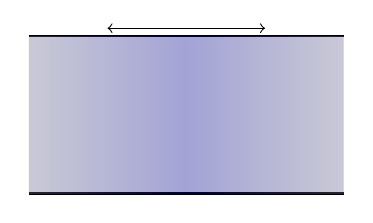
\begin{tikzpicture}
				\draw[thick] (-2,1) -- (2,1);
				\draw[thick] (-2,-1) -- (2,-1);
				\fill[left color=blue!25,right color=blue!25,middle color=blue,opacity=0.2]
				(-2,1) -- (2,1) -- (2,-1) -- (-2,-1) -- (-2,1);
				\draw[<->] (-1, 1.1) -- (1, 1.1);
			\end{tikzpicture}
		\end{center}

	\item Parallel discs -- non-uniform shear
		\begin{center}
			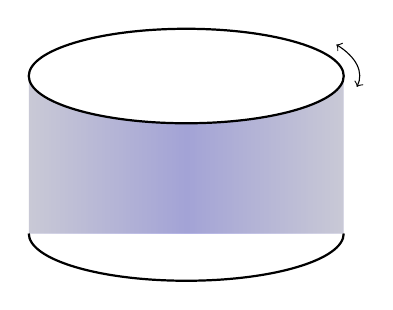
\begin{tikzpicture}
				\draw[<->] (0, 2) [partial ellipse = -10:30:2.2 and
				0.8];
				\fill[left color=blue!25,right color=blue!25,middle color=blue,opacity=0.2]
				(-2,2) -- (2,2) -- (2,0) -- (-2,0) -- (-2, 2);
				\draw[thick,fill=white] (0,2) ellipse (2 and 0.6);
				\draw[thick] (0,0) [partial ellipse = -180:0:2 and 0.6];
			\end{tikzpicture}
		\end{center}
	\item Taylor-Couette device -- non-uniform shear
		\begin{center}
			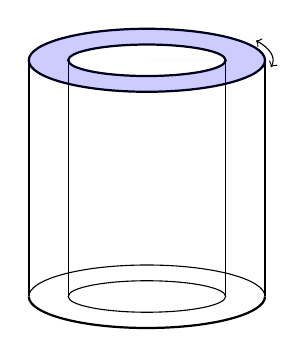
\begin{tikzpicture}
				\draw[thick,name path =A] (0,0) ellipse (1 and 0.2);
				\draw[thick,name path =B] (0,0) ellipse (1.5 and 0.4);
				\draw (0,-3) ellipse (1 and 0.2);
				\draw[thick] (0,-3) [partial ellipse = -180:0:1.5 and 0.4];
				\draw (0,-3) [partial ellipse = 0:180:1.5 and 0.4];
				\draw[<->] (0,0) [partial ellipse = -10:30:1.6 and 0.5];
				\draw[thick] (1.5,0) -- (1.5, -3);
				\draw[thick] (-1.5, 0) -- (-1.5, -3);
				\draw (1, 0) -- (1, -3);
				\draw (-1, 0) -- (-1, -3);
				\tikzfillbetween[of=A and B]{blue, opacity=0.2}
			\end{tikzpicture}
		\end{center}
	\item Cone-and-plate -- approximately uniform shear
		\begin{center}
			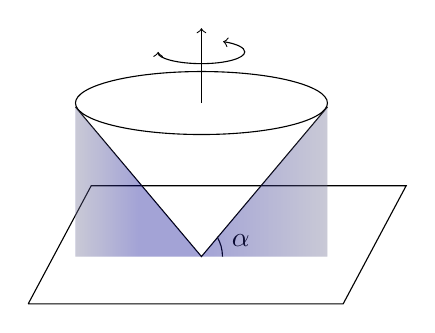
\begin{tikzpicture}
				\draw (-2,0) -- (2,0) -- (2.8, 1.5) -- (-1.2, 1.5) -- (-2,0);
				\draw (-1.4, 2.5) -- (0.2, 0.6) -- (1.8, 2.5);
				\draw (0.2, 2.55) ellipse (1.6 and 0.4);
				\draw (0.4, 0.85) arc (30:0:0.5);
				\draw (0.7, 0.8) node {$\alpha$};
				\draw[->] (0.2, 2.55) -- (0.2, 3.5);
				\draw[<->] (0.2, 3.2) [partial ellipse = -180:60:0.55 and
				0.15];
				\fill[right color = blue!25, middle color = blue, left color =
				blue, opacity=0.2] (0.2,0.6) -- (1.8, 2.5) -- (1.8,
				0.6);
				\fill[right color = blue, left color = blue!25, middle color = blue, opacity=0.2]
				(0.2,0.6) -- (-1.4, 2.5) -- (-1.4,
				0.6);
			\end{tikzpicture}
		\end{center}
\end{enumerate}

Consider oscillation with shear rate $\srate = \srate_0 \cos \omega t$ where
$\gamma_0$ is the amplitude of shear strain and $\srate_0 = \gamma_0 \omega$.
The shear stress for a GLVF is then
\begin{align}
	\sigma = \sigma(t) &= \int_{-\infty}^t G(t-t') \srate_0 \cos (\omega t' )\,
			\diffd t' \\
			&\stackrel{\mathmakebox[\widthof{=}]{s=t-t'}}{=}\srate_0 \int_0^\infty G(s) \cos
			(\omega(t-s)) \,
			\diffd s \\
			&= \srate_0 \cos \omega t \left[ \int_0^\infty G(s) \cos \omega s
		\, \diffd s \right] \\
		&+ \srate_0 \sin \omega t \left[ \int_0^\infty G(s) \sin \omega s
	\,\diffd s \right]
\end{align}
where the first term is in phase with the shear rate, and the second term is
in phase with the deformation. We can rewrite the shear stress as
\begin{equation}
	\sigma = \gamma_0 \left[ G'(\omega) \sin \omega t + G''(\omega) \cos
	\omega t \right]
\end{equation}
where
\begin{align}
	G'(\omega) &= \omega \int_0^\infty G(s) \sin \omega s \, \diffd s
						   &&\text{storage modulus} \\
	G''(\omega) &= \omega \int_0^\infty G(s) \cos \omega s \, \diffd s
							   &&\text{loss modulus}
\end{align}
The \emph{storage modulus} is analogous to the storage of elastic potential
energy in a spring, i.e. this component of the stress is a result of elastic
behaviour. Similarly, the loss modulus is analogous to the dissipation of
energy due to friction and is a result of viscous behaviour. 
\begin{itemize}
	\item The term in $G'$ has $\sigma \propto \gamma = \gamma_0 \sin \omega
		t$ and hence $G'$ is interpreted as an elastic constant, analogous to
		$k$ for a spring. 
	\item The term in $G''$ has $\sigma \propto \srate = \gamma_) \omega \cos
		\omega t$. Note that
		\begin{equation}
			\gamma_0 G''(\omega) \cos \omega t = \srate_0
			\frac{G''(\omega)}{\omega} \cos \omega t
		\end{equation}
		so we interpret $G''/\omega$ as a viscosity and define 
		\begin{equation}
			\eta'(\omega) = \frac{G''(\omega)}{\omega} = \int_0^\infty G(s)
			\cos \omega s \, \diffd s
		\end{equation}
\end{itemize}

Finally, with these definitions, we have
\begin{equation}
	\sigma = \gamma_0 G'(\omega) \sin \omega t + \srate_0 \eta'(\omega) \cos
	\omega t
\end{equation}
Note if the fluid is Newtonian, $G' = 0$ and $\eta' = \eta$. We can write $G'$
and $G''$ in a complex formulation:
\begin{equation}
	G^*(\omega) = G'' + i G' = \omega \int_0^\infty G(s) e^{i\omega s} \,
	\diffd s
\end{equation}
hence $G^*(\omega)$ is proportional to the Fourier Transform of $G(s)$.

\begin{eg}
	Consider a Maxwell fluid with $G(s) = \frac{\eta}{\lambda}e^{-s/\lambda}$.
	Then
	\begin{align}
		G^*(\omega) &= \omega \int_0^\infty \frac{\eta}{\lambda}
		e^{-s/\lambda}e^{i\omega s} \, \diffd s \\
		&= \frac{\eta \omega}{\lambda} \int_0^\infty e^{(i\omega -
		\frac{1}{\lambda})s}\,\diffd s \\
		&= - \frac{\eta \omega}{\lambda} \frac{1}{i\omega -\frac{1}{\lambda}}
		\\
		&= \frac{\eta \omega}{1-i\lambda \omega}
	\end{align}
	Taking real and imaginary parts we have
	\begin{align}
		G'(\omega) = \Im\left[G^*\right] &=
		\frac{\eta\lambda\omega^2}{1+(\lambda\omega)^2} \\
		G''(\omega) = \Re\left[ G^*\right] &= \frac{\eta\omega}{1+(\lambda\omega)^2}
	\end{align}
	\begin{center}
		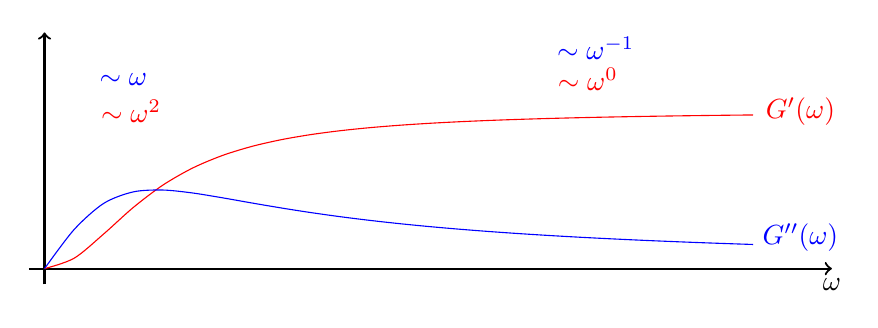
\begin{tikzpicture}[scale=2];
			\draw[thick,->] (-0.1, 0) -- (5, 0) node[right,below]
			{$\omega$};
			\draw[thick,->] (0, -0.1) -- (0, 1.5);
			\draw[red,smooth] plot[domain=0:4.5] ({\x},{2*\x*\x/(1+2*\x*\x)});
			\draw[blue,smooth] plot[domain=0:4.5] ({\x},{sqrt(2)*\x/(1+2*\x*\x)});
			\draw[red] (4.8, 1) node {$G'(\omega)$};
			\draw[blue] (4.8, 0.2) node {$G''(\omega)$};
			\draw[blue] (0.5, 1.2) node {$\sim \omega$};
			\draw[red] (0.55, 1) node {$\sim \omega^2$};
			\draw[blue] (3.5, 1.4) node {$\sim \omega^{-1}$};
			\draw[red] (3.45, 1.2) node {$\sim \omega^0$};
		\end{tikzpicture}
	\end{center}
	The maximum of $G''(x) = \frac{1}{1+x^2}$ occurs at $x=1$ hence the
	maximum of $G''(\omega)$ is at $\lambda\omega = 1$. Thus at maximum,
	$\omega = \frac{1}{\lambda}$ which can be used to estimate $\lambda$
	experimentally. We can define a new dimensionless number, the
	\emph{Deborah number} $\lambda \omega = \text{De} =
	\frac{\lambda}{\omega^{-1}}$ which is a ratio of two timescales. If
	$\text{De} \ll 1$, then $\lambda \ll \omega^{-1}$ and the Maxwell fluid
	has short memory, so an approximately Newtonian response. If $\text{De}
	\gg1 $, then $\lambda \gg\omega^{-1}$ and there are strong elastic
	effects.
\end{eg}

\subsection{Further properties}
The generalised linear visco-elastic fluid model allows modelling of fluids
with memory and history-dependent shear rate / stress relationships. However,
there are four main issues with LVFs:
\begin{enumerate}
	\item \emph{Constant viscosity in steady flow}, so the viscosity is
		independent of shear rate and we cannot model shear-thinning or
		thickening behaviour. Recall we found
		\begin{equation}
			\symbfsf{\tau} = \symbfsf{\srate}\eta
		\end{equation}
		where $\eta = \int_0^\infty G(s) \, \diffd s$.
	\item \emph{No normal stress differences.} Recall steady shear flow has
		\begin{align}
			\symbfsf{\srate} &= \begin{pmatrix} 0 & \srate & 0 \\ \srate & 0 &
			0 \\ 0 & 0 & 0 \end{pmatrix} \\
			\symbfsf{\sigma} &= \begin{pmatrix} -p_0 & \eta \srate & 0 \\ \eta
			\srate & -p_0 & 0 \\ 0 & 0 & -p_0 \end{pmatrix}
		\end{align}
		Thus $N_1 = N_2 = 0$.

	\item \emph{No change in extensional viscosity.} Recall a steady
		extensional flow has
		\begin{align}
			\symbfsf{\srate} &= \dot{\vare} \begin{pmatrix} 1 & 0 & 0 \\ 0 & 1 &
			0 \\ 0 & 0 & -2 \end{pmatrix} \\
			\symbfsf{\sigma} &= \begin{pmatrix} -p_0 + \eta \dot{\vare} & 0 &0
				\\ 0 & -p_0 + \eta \dot{\vare} & 0 \\ 0 & 0 & -p_0 - 2 \eta
			\dot{\vare} \end{pmatrix}
		\end{align}
		Hence $\eta_{\text{ext}} = 3 \eta$ and $\text{Tr} = 3$ as for a
		Newtonian fluid.

	\item The GLVF constitutive relationship is \emph{not objective}: it
		depends on the frame in which it is evaluated.
\end{enumerate}

\subsection{Frame dependence}
We have two issues to solve: translation of frame, and rotation of frame. To
solve the issue of frame translation independence, we use familiar tools from
continuum mechanics. To enforce Galilean invariance, we will use
\emph{material derivatives} instead of partial time derivatives, i.e. replace
$\partial_t$ with $\frac{\diffD}{\diffD t} = \partial_t +
\symbf{u}\cdot\nabla$.

\subsubsection{Translation}

Consider two frames of reference. Frame 1 is stationary, whilst frame 2 moves
relative to frame 1 with constant velocity $\symbf{U}$. Then
\begin{align}
	\x^{(1)} &= \x^{(2)} + \symbf{U}t \\
	\symbf{u}^{(1)} &= \symbf{u}^{(2)} + \symbf{U}
\end{align}

The stress in frame 1 and 2 may be written
\begin{align}
	\symbfsf{\sigma}^{(1)} &= \symbfsf{\sigma}^{(1)}(\x^{(1)},t) \\
	\symbfsf{\sigma}^{(2)} &= \symbfsf{\sigma}^{(2)}(\x^{(2)},t)
\end{align}
Now from Galilean invariance we have
\begin{equation}
	\symbfsf{\sigma}(\x^{(2)},t) = \symbfsf{\sigma}^{(1)}(\x^{(1)},t) =
	\symbfsf{\sigma}^{(1)}(\x^{(2)}+\symbf{U}t,t)
\end{equation}
Therefore the material derivative of $\symbfsf{\sigma}^{(2)}$ is
\begin{align}
	\frac{\diffD \symbfsf{\sigma}^{(2)}}{\diffD t} &= \frac{\partial
	\symbfsf{\sigma}^{(2)}}{\partial t} + \symbf{u}^{(2)}\cdot \nabla
	\symbfsf{\sigma}^{(2)} \\
	&= \frac{\partial}{\partial t} \left[ \symbfsf{\sigma}^{(1)}(\x^{(2)} +
\symbf{U}t,t)\right] + \symbf{u}^{(2)}\cdot\nabla \symbfsf{\sigma}^{(2)} \\
&= \frac{\partial\symbfsf{\sigma}^{(1)}}{\partial t} +
\cancel{\symbf{U}\cdot\nabla\symbfsf{\sigma}^{(1)}} +
\left(\symbf{u}^{(1)}-\cancel{\symbf{U}}\right)\cdot\nabla\symbfsf{\sigma}^{(1)}
\\
&= \frac{\diffD \symbfsf{\sigma}^{(1)}}{\diffD t}
\end{align}
Hence the material derivative is independent of the frame translation velocity
$\symbf{U}$. A Maxwell fluid previously had constitutive relationship
$\symbfsf{\sigma} +\lambda \frac{\partial \symbfsf{\sigma}}{\partial t} = \eta
\symbfsf{\srate}$. Now, we have
\begin{equation}
	\symbfsf{\sigma} + \lambda \frac{\diffD \symbfsf{\sigma}}{\diffD t} = \eta
	\symbfsf{\srate}
\end{equation}
However, this is still dependent on frame if rotation is present.

\lecture{12/11/20}
\subsubsection{Rotation}
Consider a simple shear flow on a rotating table, with lab basis vectors
$\symbf{e}_{1,2,3}$ and rotating basis vectors $\symbf{e}_{x,y,z}$.
\begin{center}
	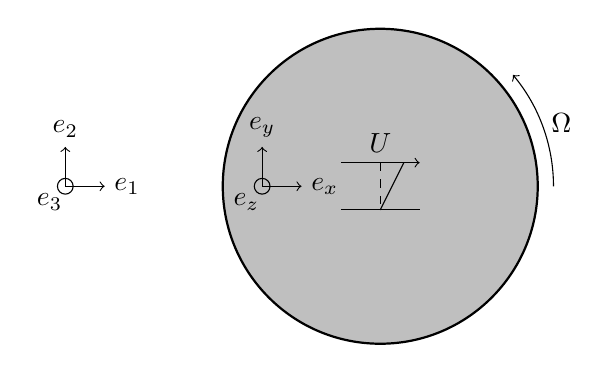
\begin{tikzpicture}
		\draw[thick,fill=gray!50] (0,0) circle (2);
		\draw[->] (2.2, 0) arc (0:40:2.2);
		\draw (2.3, 0.8) node {$\Omega$};
		\draw[->] (-0.5, 0.3) -- (0.5, 0.3) node[midway,above] {$U$};
		\draw (-0.5, -0.3) -- (0.5, -0.3);
		\draw[dashed] (0, 0.3) -- (0, -0.3);
		\draw (0,-0.3) -- (0.3,0.3);
		\draw[->] (-1.5,0) -- (-1, 0) node [right] {$\symbf{e}_x$};
		\draw[->] (-1.5,0) -- (-1.5, 0.5) node [above] {$\symbf{e}_y$};
		\draw[->] (-1.5,0) circle (0.1);
		\draw (-1.7, -0.2) node {$\symbf{e}_z$};
		\draw[->] (-4,0) -- (-3.5, 0) node [right] {$\symbf{e}_1$};
		\draw[->] (-4,0) -- (-4, 0.5) node [above] {$\symbf{e}_2$};
		\draw[->] (-4,0) circle (0.1);
		\draw (-4.2, -0.2) node {$\symbf{e}_3$};
	\end{tikzpicture}
\end{center}
If the rotation vector $\symbf{\Omega}$ is along $\symbf{e}_z$ then
\begin{equation}
	\begin{pmatrix} \symbf{e}_x(t) \\ \symbf{e}_y(t) \\ \symbf{e}_z
	\end{pmatrix} = \begin{pmatrix} \cos \Omega t & \sin \Omega t & 0 \\ -\sin
	\Omega t & \cos \Omega t & 0 \\ 0 & 0 & 1 \end{pmatrix} \begin{pmatrix}
	\symbf{e}_1 \\ \symbf{e}_2 \\ \symbf{e}_3 \end{pmatrix}
\end{equation}

Note that the two frames coincide at $t=0$. The flow has velocity $\symbf{u} =
\srate y \symbf{e}_x +$ rotation. In the table frame, the rotation does not
contribute to $\symbfsf{\srate}$ so we have
\begin{align}
	\symbfsf{\srate} &= \begin{pmatrix} 0 & \srate & 0 \\ \srate & 0 & 0 \\ 0 &
	0 & 0 \end{pmatrix} = \srate (\symbf{e}_x\symbf{e}_y +
	\symbf{e}_y\symbf{e}_x) \\
	\implies \symbfsf{\tau} &= \int_{-\infty}^t G(t-t') \symbfsf{\srate} \,
	\diffd t' = \symbfsf{\srate} \int_{-\infty}^t G(t-t')\,\diffd t' =
	\eta_{\{x,y\}} \symbfsf{\srate}
\end{align}
where for any linear viscoelastic fluid,
\begin{equation}
	\eta_{\{x,y\}} = \int_0^\infty G(s) \, \diffd s
\end{equation}
In the lab frame, we use the expressions for $\symbf{e}_{x,y,z}$ in terms of
$\symbf{e}_{1,2,3}$ to get
\begin{align}
	\symbfsf{\srate} &= \srate (\symbf{e}_x\symbf{e}_y +
	\symbf{e}_y\symbf{e}_x) \\
	&= \srate \begin{pmatrix} -\sin(2\Omega t) & \cos(2\Omega t) & 0 \\
\cos(2\Omega t) & \sin(2\Omega t) & 0 \\ 0 & 0 & 0 \end{pmatrix}
\end{align}
with respect to the $\symbf{e}_{1,2,3}$ basis. The relevant deviatoric stress
$\symbfsf{\tau}_{12}$ in the lab frame is then
\begin{align}
	\symbfsf{\tau}_{12} &= \int_{-\infty}^t G(t-t') \srate \cos 2 \Omega t' \,
	\diffd t' \\
	&\stackrel{\mathmakebox[\widthof{=}]{s=t-t'}}{=} \int_0^\infty G(s) \srate
	\cos 2 \Omega (t-s) \, \diffd s
\end{align}

At $t=0$, both frames coincide so we expect the viscosity is the same in both
frames at this time. We find
\begin{equation}
	\left.\symbfsf{\tau}_{12}\right|_{t=0} = \srate \int_0^\infty G(s) \cos 2
		\Omega s \, \diffd s = \eta_{\{1,2\}}\srate
\end{equation}
where $\eta_{\{1,2\}} = \int_0^\infty G(s)\cos 2\Omega s \, \diffd s \ne
\eta_{\{x,y\}}$. Hence we find the viscosity depends on the frame used to
evaluate it. This is a fundamental problem with the LVF constitutive
relaetionship. We can fix this by introducing \emph{objective derivatives} for
tensors.  Note $G(s)$ has support when $s = \mathcal{O}(\lambda)$. Therefore
in the integral for $\eta_{\{1,2\}}$, if $\Omega \lambda \ll 1$ then $\cos 2
\Omega s \sim 1$ so the viscosities agree. Hence we can use the LVF model for
flows with small velocity gradients or very short memory.

\section{Objective Derivatives}
\subsection{Oldroyd's axioms}
Newtonian fluid mechanics was developed in the 19\textsuperscript{th} century.
The theory of complex fluids was developed in the 20\textsuperscript{th}
century. In the 1950s, there was intense research to set up a rigorous
mathematical framework for continuum mechanics. There are two different
approaches:
\begin{itemize}
	\item \emph{Bottom up:} start with a microscopic model and from this form
		field equations via averaging. For example, polymers, statistical
		physics, ensemble avergaging gives field equations for density and
		velocity.
	\item \emph{Top down:} axiomatic approach. Consider all terms that are
		admissible in a hydrodynamic equation based on symmetries or
		invariance principles. Fit the resulting free parameters to
		experimental data.
\end{itemize}

The game changer was Professor James Oldroyd who specified four axioms a
constitutive equation must satisfy. A constitutive relationship must be based
on:
\begin{enumerate}
	\item the relative motion of the neighbourhood of the (current) particle;
	\item the history of the strain tensor associated with the particles;
	\item physical constants defining the behaviour of the material (and obey
		its symmetries);
	\item a \emph{convective} coordinate system that is \emph{embedded} in the
		material and is \emph{deforming} with it, i.e. can only involve
		derivatives that do not depend on the frame where they are evaluated
		but instead need to be \emph{intrinsic}.
\end{enumerate}

Thus far, we have satisfied the first three axioms. Axiom 4 requires the
introduce of `new' tensor derivatives.

\subsection{Upper-convected derivative}
Consider two frames.
\begin{enumerate}
	\item The `lab' Cartesian frame with basis vectors $\symbf{e}_i$ and
		coordinates $x_i$.
	\item Curvilinear coordinates deforming with the flow (\emph{covariant})
		with basis vectors $\symbf{g}_j$ and coordinates $a_j$.
\end{enumerate}
\begin{center}
	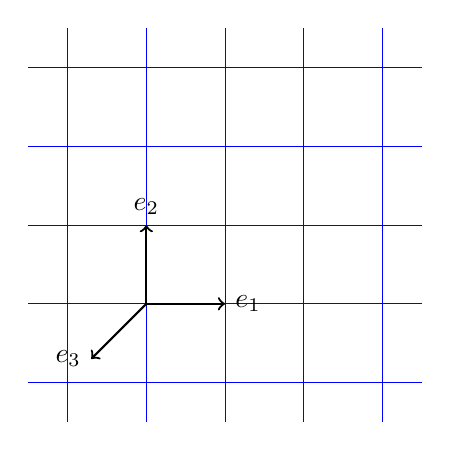
\begin{tikzpicture}
		\draw[step=1,blue,thin] (0.5,0.5) grid (5.5,5.5);
		\draw[thick,->](2,2) -- (3,2) node[right] {$\symbf{e}_1$};
		\draw[thick,->](2,2) -- (2,3) node[above] {$\symbf{e}_2$};
		\draw[thick,->] (2,2) -- (1.3, 1.3) node[left] {$\symbf{e}_3$};
	\end{tikzpicture}
	\qquad
	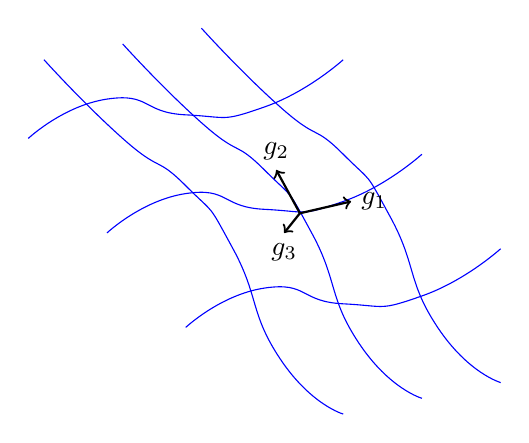
\begin{tikzpicture}
		\foreach \off in {0,1,2} {
			\draw[blue,thin] plot[smooth,tension=1] coordinates
			{(0+\off,0-1.2*\off) (1+\off,0.5-1.2*\off) (2+\off,0.3-1.2*\off)
		(3+\off, 0.4-1.2*\off) (4+\off,1-1.2*\off)} ;};
		\foreach \off in {0,1,2} {
			\draw[blue,thin] plot[smooth,tension=1] coordinates
			{(0.2+\off,1+0.2*\off) (1.2+\off, 0+0.2*\off) (2+\off,
			-0.6+0.2*\off) (2.6+\off, -1.4+0.2*\off) (3.2+\off, -2.8+0.2*\off)
			(4+\off, -3.5+0.2*\off)};
		 };
		 \draw[thick,->] (3.45, -0.95) -- (4.1, -0.8) node[right]
		 {$\symbf{g}_1$};
		 \draw[thick,->] (3.45, -0.95) -- (3.15, -0.4) node[above]
		 {$\symbf{g}_2$};
		 \draw[thick,->] (3.45, -0.95) -- (3.25, -1.2) node[below]
		 {$\symbf{g}_3$};
	\end{tikzpicture}
\end{center}

The covariant vectors $\symbf{g}_i$ are \emph{material vectors}, meaning they
may change in length and orientation with the deforming material. The stress
tensor in each frame is
\begin{equation}
	\symbfsf{\sigma} = \begin{cases} \sigma_{mn} \symbf{e}_m \symbf{e}_n &
		\text{lab frame} \\ \hat{\sigma}_{ij} \symbf{g}_i \symbf{g}_j &
		\text{covariant frame}
	\end{cases}
\end{equation}

A material point $\symbf{x}$ is represented as $\symbf{x} = x_j \symbf{e}_j$
in the lap frame and $\symbf{x} = a_j \symbf{g}_j$ in the covariant frame.
Hence by definition
\begin{equation}
	\symbf{g}_i = \frac{\partial \symbf{x}}{\partial a_i} =
	\frac{\partial}{\partial a_i} \left[ x_j \symbf{e}_j\right] =
	\frac{\partial x_j}{\partial a_i} \symbf{e}_j
\end{equation}
Define the \emph{deformation gradient tensor} $\symsf{F}$ such that
\begin{equation}
	\symsf{F}_{ij} = \frac{\partial x_j}{\partial a_i}
\end{equation}
Then $\symbf{g}_i = F_{ij} \symbf{e}_j$. Using this frame transformation rule,
we can form a tensor transformation rule for $\symbfsf{\sigma}$:
\begin{align}
	\symbfsf{\sigma} = \sigma_{mn} \symbf{e}_m \symbf{e}_n &= \hat{\sigma}_{ij}
	\symbf{g}_i \symbf{g}_j  \\
	&= \hat{\sigma}_{ij} F_{im} F_{jn} \symbf{e}_m \symbf{e}_n \\
	\implies \sigma_{mn} &= \hat{\sigma}_{ij} F_{im} F_{jn}
\end{align}
In tensor notation, this is equivalent to
\begin{equation}
	\symbfsf{\sigma} = \symsf{F}^T \cdot \hat{\symbfsf{\sigma}} \cdot
	\symsf{F} \iff \hat{\symbfsf{\sigma}} = \left( \symsf{F}^T\right)^{-1}
	\cdot \symbfsf{\sigma} \cdot \symsf{F}^{-1}
\end{equation}
Note that $\symsf{F}$ is not unitary. We can now calculate the
\emph{intrinsic} time derivative of $\hat{\symbfsf{\sigma}}$:
\begin{align}
	\frac{\diffD}{\diffD t} \hat{\symbfsf{\sigma}} &= \frac{\diffD}{\diffD t}
	\left[ \symsf{F}^{-T} \cdot \symbfsf{\sigma} \cdot \symsf{F}^{-1}\right]
	\\
	&= \left( \frac{\diffD}{\diffD t} \symsf{F}^{-T}\right) \cdot
	\symbfsf{\sigma} \cdot \symsf{F}^{-1} + \symsf{F}^{-T} \cdot \left(
	\frac{\diffD}{\diffD t} \symbfsf{\sigma}\right) \cdot \symsf{F}^{-1} +
	\symsf{F}^{-T} \cdot \symbfsf{\sigma}  \cdot \left( \frac{\diffD}{\diffD
	t} \symsf{F}^{-1}\right)
\end{align}
To elucidate this expression we wish to calculate the material derivative of
$\symsf{F}$, using the fact $x_j = x_j(a_i,t)$ so we can commute
$\frac{\diffD}{\diffD t}$ with $\frac{\partial}{\partial a_i}$. We find
\begin{align}
	\frac{\diffD}{\diffD t} \symsf{F}_{ij} = \frac{\diffD}{\diffD t}
	\frac{\partial x_j}{\partial a_i} = \frac{\partial}{\partial a_i}
	\frac{\diffD x_j}{\diffD t} &= \frac{\partial u_j}{\partial a_i} \\
						&=
	\frac{\partial u_j}{\partial x_k} \frac{\partial x_k}{\partial a_i} \\
	&= \symsf{F}_{ik} \left(\nabla \symbf{u}\right)_{kj}\\
	\therefore\,\,\, \frac{\diffD}{\diffD t} \symsf{F} &= \symsf{F} \cdot \nabla
	\symbf{u}
\end{align}
Now we know $\symsf{F} \cdot \symsf{F}^{-1} = \symsf{I}$, hence
\begin{align}
	\frac{\diffD \symsf{F}}{\diffD t} \cdot \symsf{F}^{-1} + \symsf{F} \cdot
	\frac{\diffD \symsf{F}^{-1}}{\diffD t} &= 0 \\
	\implies \frac{\diffD \symsf{F}^{-1}}{\diffD t} &= - \symsf{F}^{-1} \cdot
	\frac{\diffD \symsf{F}}{\diffD t} \cdot \symsf{F}^{-1} = -(\nabla
	\symbf{u})\cdot\symsf{F}^{-1}\\
	\frac{\diffD \symsf{F}^{-T}}{\diffD t} &= - \symsf{F}^{-T} \cdot (\nabla
	\symsf{u})^T
\end{align}

Collecting these results we have
\begin{equation}
	\frac{\diffD \hat{\symbfsf{\sigma}}}{\diffD t} = \symsf{F}^{-T} \cdot
	\left[ \frac{\diffD \symbfsf{\sigma}}{\diffD t} - (\nabla \symbf{u})^T
		\cdot \symbfsf{\sigma} - \symbfsf{\sigma} \cdot (\nabla
	\symbf{u})\right] \cdot \symsf{F}^{-1}
\end{equation}
This is in the form of the frame transformation rule for tensors. Hence the
intrinsic derivative of the stress tensor in the lab basis is
\begin{equation}
	\stackrel{\bigtriangledown}{\symbfsf{\sigma}}\, = \frac{\diffD
		\symbfsf{\sigma}}{\diffD t} - (\nabla \symbf{u})^T \cdot
		\symbfsf{\sigma} - \symbfsf{\sigma} \cdot (\nabla \symbf{u})
\end{equation}
This is the \emph{upper-convected derivative} (UCD) which is objective, i.e.
independent of frame. It is the derivative measured intrinsically as it
deforms with the flow. Note that
\begin{equation}
	\stackrel{\bigtriangledown}{\symsf{I}} = 0 - (\nabla \symbf{u})^T\cdot
	\symsf{I} - \symsf{I}\cdot (\nabla \symbf{u}) = -\symbfsf{\srate}
\end{equation}

Other ways of defining objective derivatives include
\begin{itemize}
	\item \emph{Lower-convected derivative}
		\begin{equation}
			\stackrel{\bigtriangleup}{\symbfsf{\sigma}} = \frac{\diffD
		\symbfsf{\sigma}}{\diffD t} + (\nabla \symbf{u})^T \cdot
		\symbfsf{\sigma} + \symbfsf{\sigma} \cdot (\nabla \symbf{u})
	\end{equation}
	\item \emph{Co-rotational derivative}
		\begin{equation}
			\frac{\mathcal{D} \symbfsf{\sigma}}{\mathcal{D} t} = \frac{\diffD
				\symbfsf{\sigma}}{\diffD t} + \frac{1}{2} \left(
				\symbf{\omega}\cdot\symbfsf{\sigma} -
			\symbfsf{\sigma}\cdot\symbf{\omega}\right)
		\end{equation}
		where $\symbf{\omega} = \nabla \symbf{u} - (\nabla \symbf{u})^T$.
\end{itemize}

\lecture{17/11/20}
\section{Retarded Motion Expansion}
\subsection{Ordered Fluids}
Here we consider our first non-linear model of complex fluids. We consider an
expansion about Newtonian fluid behaviour where successive terms account
systematically for deviations from Newtonian behaviour due to elastic effects.
This is a popular model to carry out rigorous mathematical analysis of
\emph{weakly non-Newtonian flows}. Also, this is a popular model to obtain
physical insight. However, the model is not very practical because it is
limited to small deformations.

We will consider a Taylor expansion of deviatoric stress $\symsf{\tau} =
f(\nabla \symbf{u})$ as a function of $\nabla \symbf{u}$. We assume four
properties:
\begin{enumerate}
	\item Incompressibility $\nabla\cdot\symbf{u} = 0$.
	\item Deviatoric stress $\symsf{\tau}$ is symmetric.
	\item Deviatoric stress $\symsf{\tau}$ is objective.
	\item As in a standard Taylor expansion, assume $\symsf{\tau}$ has
		polynomial dependence on deformation.
\end{enumerate}

Define the \emph{$n$\textsuperscript{th} shear rate tensor}
$\symsf{\gamma}_{(n)}$ by
\begin{align}
	\symbfsf{\gamma}_{(1)} &= \symbfsf{\srate} && \text{shear rate tensor, linear in}
	\,\,\, \nabla \symbf{u} \\
	\symbfsf{\gamma}_{(2)} &=
	\stackrel{\bigtriangledown}{\symbfsf{\gamma}}_{(1)} &&
	\text{2\textsuperscript{nd} shear rate tensor, quadratic in}
	\,\,\, \nabla \symbf{u} \\
	&\vdots \\
	\symbfsf{\gamma}_{(n)} &=
	\stackrel{\bigtriangledown}{\symbfsf{\gamma}}_{(n-1)} &&
	\text{n\textsuperscript{th} shear rate tensor, proportional to}
	\,\,\, \abs{\nabla \symbf{u}}^n \\
\end{align}

An \emph{ordered fluid} is one in which we collect terms in the expansion of
the same order in $\nabla \symbf{u}$, then truncate. This is the
\emph{retarded motion expansion}.

A first-order fluid, linear in $\nabla \symbf{u}$, has
\begin{equation}
	\symbfsf{\tau}^{(1)} = c \symbfsf{\gamma}_{(1)} = c \symbfsf{\srate}
\end{equation}
Hence a first-order fluid is Newtonian with $\eta = c$. A second-order fluid,
quadratic in $\nabla \symbf{u}$, has
\begin{equation}
	\symbfsf{\tau}^{(2)} = b_1 \symbfsf{\gamma}_{(1)} + b_2
	\symbfsf{\gamma}_{(2)} +
	b_{11} \symbfsf{\gamma}_{(1)} \cdot \symbfsf{\gamma}_{(1)}
\end{equation}
where the first term is linear and the second two terms are quadratic in
$\nabla \symbf{u}$. For higher order fluids, the number of free parameters
increases combinatorially. For example, a 3\textsuperscript{rd} order fluid
has 6 free parameters
\begin{equation}
	\symbfsf{\tau}^{(3)} = \symbfsf{\tau}^{(2)} + b_3 \symbfsf{\gamma}_{(3)} +
	b_{12} \left[ \symbfsf{\gamma}_{(1)}\cdot\symbfsf{\gamma}_{(2)} +
	\symbfsf{\gamma}_{(2)} \cdot \symbfsf{\gamma}_{(1)}\right] + b_{1:11}
	(\symbfsf{\gamma}_{(1)}\cdot
	\symbfsf{\gamma}_{(1)})\cdot\symbfsf{\gamma}_{(1)}
\end{equation}
These ordered fluids are \emph{admissible} from the point of view of continuum
mechanics. We need to supplement the model with microscopic models (e.g.
kinetic theory) to give values,s igns, etc, for free parameters. This is an
example of a bottom up approach. For example, we find
\begin{enumerate}
	\item $b_1 > 0$
	\item $b_n$ alternate in sign
	\item For a second-order fluid, $\abs{b_2} > \abs{b_1}$.
\end{enumerate}

\subsection{Shear flow of second-order fluid.}
We have three free parameters $b_1, b_2, b_{11}$ for which we want to gain a
physical interpretation. For a simple shear flow with $\symbf{u} = \srate y
\hat{\symbf{x}}$ we have
\begin{equation}
	\symbfsf{\gamma}_{(1)} = \symbfsf{\srate} = \begin{pmatrix} 0 & \srate & 0 \\
	\srate & 0 & 0 \\ 0 & 0 & 0 \end{pmatrix}, \hspace{2em} \nabla \symbf{u} =
\begin{pmatrix} 0 & 0 & 0 \\ \srate & 0 & 0 \\ 0 & 0 & 0 \end{pmatrix}
\end{equation}

Now using the upper-convected derivative the second shear rate tensor is
\begin{align}
	\symbfsf{\gamma}_{(2)} =
	\stackrel{\bigtriangledown}{\symbfsf{\gamma}}_{(1)} &=
	\cancel{\frac{\diffD}{\diffD t} \symbfsf{\gamma}_{(1)}} - (\nabla \symbf{u})^T
	\cdot \symbfsf{\gamma}_{(1)} - \symbfsf{\gamma}_{(1)} \cdot (\nabla \symbf{u} )\\
	&= - (\nabla \symbf{u})^T \cdot \symbfsf{\gamma}_{(1)} -
	\symbfsf{\gamma}_{(1)}\cdot (\nabla \symbf{u}) \\
	&= \begin{pmatrix} - 2\srate^2 & 0 & 0 \\ 0 & 0 & 0 \\ 0 & 0 & 0
	\end{pmatrix}
\end{align}
where the material derivative vanishes since we have a steady and spatially
uniform shear rate tensor. Hence
\begin{equation}
	\symbfsf{\tau} = \begin{pmatrix} b_{11} \srate^2 - 2b_2 \srate^2 & b_1
		\srate & 0 \\ b_1 \srate & b_{11} \srate^2 & 0 \\ 0 & 0 & 0
	\end{pmatrix}
\end{equation}

As a consistency check, note that to get Newtonian behaviour we require
$b_{11} = b_2 = 0$, i.e. the non-Newtonian terms vanish. If $(b_{11}, b_2) \ne
(0,0)$ we get new non-Newtonian behaviour. The shear stress $\tau_{xy} = b_1
\srate$ hence we have constant viscosity $\eta = b_1$. Since we are dealing
with steady shear, normal stress differences are defined:
\begin{align}
	N_1 &= \tau_{xx} - \tau_{yy} = -2b_2 \srate^2 = \Psi_1 \srate^2 \\
	N_2 &= \tau_{yy} - \tau_{zz} = b_{11} \srate^2 = \Psi_2 \srate^2 \\
\end{align}
where $\Psi_1, \Psi_2$ are the normal stress coefficients. Hence $\Psi_1 =
-2b_2, \Psi_2 = b_{11}$ i.e. we have constant first and second normal stress
coefficients.  Note $b_1, b_2, b_{11}$ (i.e. $\eta, \Psi_1, \Psi_2$) are
material constants.  We now rewrite the constitutive relationship using
material parameters, which can be measured.
\begin{equation}
	\symbfsf{\tau} = \eta \symbfsf{\srate} - \frac{1}{2} \Psi_{1}
	\stackrel{\bigtriangledown}{\symbfsf{\srate}} + \Psi_2
	\symbfsf{\srate}\cdot\symbfsf{\srate}
\end{equation}

\paragraph{Physical intuition.}
Recall $\Psi_1 > 0, \Psi_2 < 0$ and $\abs{\Psi_2/\Psi_1}$ is small. We now use
this calculation to get a physical intuition for the behaviour of a second
order fluid. Consider
\begin{equation}
	\symbfsf{\tau}_{xx} = (b_{11} - 2b_2) \srate^2 = (\Psi_1 + \Psi_2)
	\srate^2 > 0
\end{equation}
since $\Psi_1$ dominates and is positive. Hence $\symbfsf{\tau}_{xx}$ is
elastic tension, resisting motion. Also,
\begin{equation}
	\symbfsf{\tau}_{yy} = \Psi_2 \srate^2 < 0
\end{equation}
hence $\symbfsf{\tau}_{yy}$ is a normal elastic force, acting to separate the
plates. The units of the three free parameters are
\begin{align}
	\left[ b_1\right] &= \left[ \eta \right] = \text{stress} \times \text{time}
	\\
	\left[b_2, b_{11} \right] &= \text{stress} \times \text{time}^2
\end{align}
Hence $b_2/b_1 = \Psi_1 / \eta$ is a timescale, which is in fact a good
estimate for relaxation time $\lambda$.

\paragraph{Model validity.}
When do we expect the second-order fluid model to remain valid? For validity,
we require the second order terms to be a small perturbation to the first
order terms. Hence
\begin{equation}
	\abs{\frac{b_2 \symbfsf{\gamma}_{(2)}}{b_1 \symbfsf{\gamma}_{(1)}}} \ll 1
\end{equation}
The scalings for the appropriate terms are
\begin{align}
	\abs{\symbfsf{\srate}} &\sim \srate\\
	\abs{b_2 \symbfsf{\gamma}_{(2)}} &\sim \Psi_1 \srate^2 \\
	\abs{b_1 \symbfsf{\gamma}_{(1)}} &\sim \eta \srate
\end{align}
Hence for validity we require
\begin{equation}
	\frac{\Psi_1 \srate^2}{\eta \srate} \ll 1 \implies \lambda \srate \ll 1
\end{equation}
Now define a new dimensionless number $\text{Wi} = \lambda \srate$, the
\emph{Weissenberg number}. $\text{Wi} = \lambda / (1/\srate)$ is a ratio of
timescales for relaxation and deformation. This is a ratio of \emph{intrinsic}
timescales to \emph{flow} timescales, which thus measures the relative
importance of elastic effects in the fluid.  Ordered fluids are expansions
valid asymptotically in the limit $\text{Wi} \to 0$.


\end{document}
